% =====================================================================
%  Connecting an HPC Language Model to a Local CarlaAir Simulator
%  A verified manual for ERAU Vega
%  Compile:  pdflatex -interaction=nonstopmode vega-carlaair-manual.tex
%            (run twice so the table of contents and references resolve)
% =====================================================================
\documentclass[11pt,a4paper]{article}

\usepackage[T1]{fontenc}
\usepackage[utf8]{inputenc}
\usepackage{lmodern}
\usepackage[margin=2.3cm]{geometry}
\usepackage{booktabs}
\usepackage{tabularx}
\usepackage{longtable}
\usepackage{array}
\usepackage{xcolor}
\usepackage{enumitem}
\usepackage{fancyhdr}
\usepackage{titlesec}
\usepackage{caption}
\usepackage{listings}
\usepackage{tikz}
\usetikzlibrary{positioning,arrows.meta,shapes.geometric,calc,fit,backgrounds,decorations.pathreplacing}
\usepackage[normalem]{ulem}
\usepackage[hidelinks]{hyperref}

% ---------------------------------------------------------------- colours
\definecolor{ink}{HTML}{1A1A1A}
\definecolor{accent}{HTML}{1F4E79}
\definecolor{accent2}{HTML}{C0504D}
\definecolor{good}{HTML}{2E7D32}
\definecolor{warn}{HTML}{B36B00}
\definecolor{shade}{HTML}{F2F4F7}
\definecolor{rule}{HTML}{C8CDD4}
\definecolor{laptop}{HTML}{E8F0FA}
\definecolor{cluster}{HTML}{FBECEC}

% ---------------------------------------------------------------- styling
\titleformat{\section}{\Large\bfseries\color{accent}}{\thesection}{0.7em}{}
\titleformat{\subsection}{\large\bfseries\color{ink}}{\thesubsection}{0.6em}{}
\titleformat{\subsubsection}{\normalsize\bfseries\color{ink}}{\thesubsubsection}{0.5em}{}
\setlist[itemize]{leftmargin=1.3em,topsep=3pt,itemsep=2pt}
\setlist[enumerate]{leftmargin=1.5em,topsep=3pt,itemsep=2pt}
\captionsetup{font=small,labelfont={bf,color=accent}}

\pagestyle{fancy}
\fancyhf{}
\fancyhead[L]{\small\color{accent}HPC $\rightarrow$ CarlaAir: a verified manual}
\fancyhead[R]{\small\thepage}
\renewcommand{\headrulewidth}{0.4pt}

% ---------------------------------------------------------------- code
\lstdefinestyle{sh}{
  basicstyle=\ttfamily\small,
  backgroundcolor=\color{shade},
  frame=single, rulecolor=\color{rule},
  framesep=5pt, xleftmargin=6pt, xrightmargin=2pt,
  breaklines=true, breakatwhitespace=false,
  postbreak=\mbox{\textcolor{accent2}{$\hookrightarrow$}\space},
  showstringspaces=false, keepspaces=true,
  columns=fullflexible, literate={~}{{\textasciitilde}}1,
}
\lstset{style=sh}
\newcommand{\cmd}[1]{\texttt{\small #1}}

% ---------------------------------------------------------------- callouts
\newcommand{\callout}[3]{%
  \par\medskip\noindent
  \begin{tikzpicture}
    \node[inner sep=7pt, align=left, text width=\dimexpr\linewidth-20pt\relax,
          fill=#1!7, draw=#1, line width=0.9pt, rounded corners=2pt] (box)
      {\textbf{\color{#1}#2}\\[2pt]#3};
  \end{tikzpicture}\par\medskip}

\newcommand{\verified}{{\color{good}\textbf{[verified]}}}
\newcommand{\untested}{{\color{warn}\textbf{[not exercised]}}}

% =====================================================================
\begin{document}

\begin{titlepage}
\centering
\vspace*{2.2cm}
{\color{accent}\rule{\linewidth}{1.4pt}}\\[6pt]
{\Huge\bfseries Connecting an HPC Language Model\\[6pt] to a Local CarlaAir Simulator\par}
\vspace{10pt}
{\color{accent}\rule{\linewidth}{1.4pt}}\\[18pt]
{\Large A verified manual for ERAU Vega\par}
\vspace{6pt}
{\large Agentic UAV coordination study --- open-loop baseline\par}
\vfill

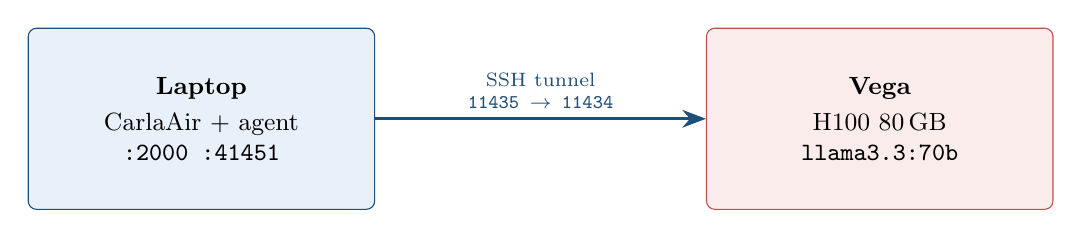
\begin{tikzpicture}[font=\small]
  \node[draw=accent, fill=laptop, rounded corners=3pt, minimum width=4.4cm,
        minimum height=2.3cm, align=center] (lap)
    {\textbf{Laptop}\\[2pt] CarlaAir + agent\\ \texttt{:2000 :41451}};
  \node[draw=accent2, fill=cluster, rounded corners=3pt, minimum width=4.4cm,
        minimum height=2.3cm, align=center, right=4.2cm of lap] (hpc)
    {\textbf{Vega}\\[2pt] H100 80\,GB\\ \texttt{llama3.3:70b}};
  \draw[-{Stealth[length=3mm]}, line width=1pt, accent]
    (lap.east) -- node[above, align=center, font=\scriptsize]
    {SSH tunnel\\ \texttt{11435 $\rightarrow$ 11434}} (hpc.west);
\end{tikzpicture}

\vfill
{\large Aditya Chikhaliya\par}
{\small Embry--Riddle Aeronautical University\par}
\vspace{4pt}
{\small Setup performed 6 October 2026 \quad$\cdot$\quad revised 20 October 2026\par}
\vspace{10pt}
{\footnotesize Every command marked \verified{} was run on Vega and its output observed.\\
Commands marked \untested{} are documented but not yet exercised.\par}
\end{titlepage}

\tableofcontents
\newpage

% =====================================================================
\section{What this manual is}

This manual records how a large language model running on a university
supercomputer was connected to a flight simulator running on a laptop, so that
the simulator could ask the model to plan missions for uncrewed aerial vehicles.

It is written from a working installation rather than from documentation. Where
the official documentation is wrong, this says so and gives what actually
worked. Where something was never tested, it says that too, because a manual
that cannot distinguish the two is not trustworthy.

\callout{accent}{The one-sentence version}{%
Run \texttt{ollama serve} inside a GPU job on Vega bound to \texttt{0.0.0.0:11434},
open an SSH tunnel from the laptop that forwards local port \textbf{11435} to that
node's 11434 through the login node, and point the agent at
\texttt{http://127.0.0.1:11435}.}

\subsection{Who it is for}

Someone who has an ERAU account, a laptop that runs the simulator, and no prior
experience of high-performance computing. Every term is defined at first use and
collected in the glossary in Section~\ref{sec:glossary}.

\subsection{The problem being solved}

The research question is how a language model's capability affects the quality
of flight plans it produces. Answering it needs models of different sizes. A
laptop with 4\,GB of video memory can run a 3-billion-parameter model; a
70-billion-parameter model needs roughly 42\,GB and will not fit. Vega has
H100 GPUs with 80\,GB each.

So the model must move to the cluster. The simulator cannot: CarlaAir is a
Windows build that needs a graphics display, and the cluster is a headless Linux
system. The two halves therefore have to run on different machines and talk to
each other, which is what the rest of this manual is about.

% =====================================================================
\section{The architecture, and why it is sound}

\subsection{What runs where}

\begin{figure}[h]
\centering
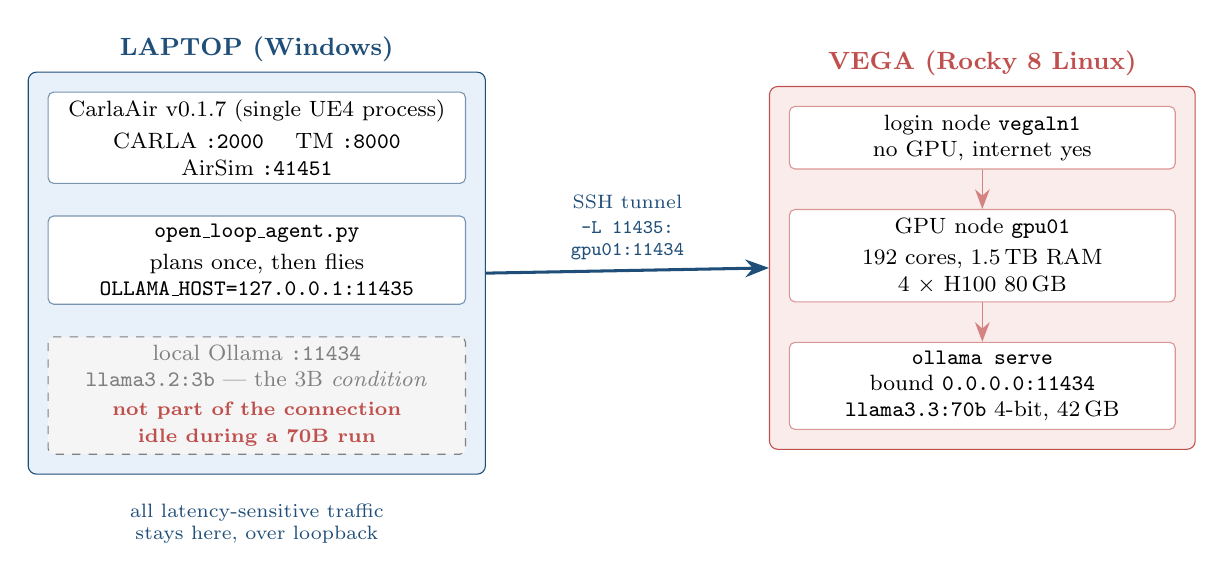
\begin{tikzpicture}[font=\footnotesize,
  lbox/.style={draw=accent!60, fill=white, rounded corners=2pt,
               minimum width=5.3cm, align=center, inner sep=3pt},
  rbox/.style={draw=accent2!60, fill=white, rounded corners=2pt,
               minimum width=4.9cm, align=center, inner sep=3pt}]

% ---- laptop column. Each node is placed relative to the one above it, and the
% container is fitted around them afterwards, so no box can outgrow its frame.
\node[lbox] (carla)
  {CarlaAir v0.1.7 (single UE4 process)\\[2pt]
   CARLA \texttt{:2000} \quad TM \texttt{:8000}\\ AirSim \texttt{:41451}};
\node[lbox, below=4mm of carla] (agent)
  {\texttt{open\_loop\_agent.py}\\[2pt]
   plans once, then flies\\
   \texttt{OLLAMA\_HOST=127.0.0.1:11435}};
\node[lbox, draw=gray, dashed, fill=gray!8, below=4mm of agent] (localollama)
  {\textcolor{gray}{local Ollama \texttt{:11434}}\\
   \textcolor{gray}{\texttt{llama3.2:3b} --- the 3B \emph{condition}}\\[1pt]
   \textcolor{accent2}{\scriptsize\textbf{not part of the connection}}\\
   \textcolor{accent2}{\scriptsize\textbf{idle during a 70B run}}};

% ---- cluster column
\node[rbox, right=4.1cm of carla] (login)
  {login node \texttt{vegaln1}\\ no GPU, internet yes};
\node[rbox, below=5mm of login] (gpunode)
  {GPU node \texttt{gpu01}\\[2pt] 192 cores, 1.5\,TB RAM\\ 4 $\times$ H100 80\,GB};
\node[rbox, below=5mm of gpunode] (serve)
  {\texttt{ollama serve}\\ bound \texttt{0.0.0.0:11434}\\ \texttt{llama3.3:70b} 4-bit, 42\,GB};

\draw[-{Stealth[length=2.5mm]}, accent2!70] (login) -- (gpunode);
\draw[-{Stealth[length=2.5mm]}, accent2!70] (gpunode) -- (serve);

\begin{scope}[on background layer]
  \node[draw=accent, fill=laptop, rounded corners=3pt, inner sep=7pt,
        fit=(carla)(agent)(localollama),
        label={[font=\small\bfseries, text=accent]above:LAPTOP (Windows)}] (lapbox) {};
  \node[draw=accent2, fill=cluster, rounded corners=3pt, inner sep=7pt,
        fit=(login)(gpunode)(serve),
        label={[font=\small\bfseries, text=accent2]above:VEGA (Rocky 8 Linux)}] (hpcbox) {};
\end{scope}

% ---- the tunnel, drawn between the two containers so the label has the whole
% gap to itself rather than sitting on a box edge.
\draw[-{Stealth[length=3mm]}, line width=1.1pt, accent]
  (lapbox.east) -- node[above, font=\scriptsize, align=center]
  {SSH tunnel\\[1pt] \texttt{-L 11435:}\\ \texttt{gpu01:11434}} (hpcbox.west);

\node[font=\scriptsize, text=accent, below=2.5mm of lapbox.south, align=center]
  {all latency-sensitive traffic\\ stays here, over loopback};
\end{tikzpicture}
\caption{What runs where. Only the planning request crosses the network. The
simulator, the agent's control loop, pose reads and the separation monitor all
stay on the laptop over the loopback interface. \textbf{The greyed box is not
infrastructure} --- the laptop's own Ollama is a \emph{condition being measured}
(Section~\ref{sec:threecopies}) and sits idle while the 70B is in use. It is
drawn because it is there, and because it occupies port 11434, which is why the
tunnel uses 11435.}
\label{fig:arch}
\end{figure}

\subsection{Why splitting the system does not corrupt the measurements}

This is the part that makes the architecture defensible rather than merely
convenient.

The baseline agent is \textbf{open loop}. It asks the model for a complete plan
\emph{before the aircraft leaves the ground}, validates that plan against a
schema, and then executes it without ever consulting the model again. So:

\begin{itemize}
  \item exactly one network request happens per drone per mission;
  \item it happens while the aircraft is stationary on the ground;
  \item network latency therefore cannot affect flight timing, control
        stability, or the separation between drones.
\end{itemize}

\begin{figure}[h]
\centering
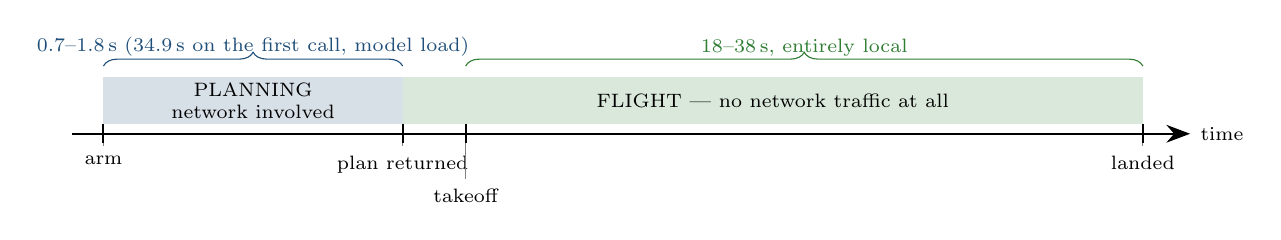
\begin{tikzpicture}[font=\footnotesize]
  \draw[-{Stealth[length=3mm]}, line width=0.9pt] (0,0) -- (14.2,0)
    node[right, font=\scriptsize] {time};

  % phases
  \fill[accent!18] (0.4,0.12) rectangle (4.2,0.72);
  \node[font=\scriptsize, align=center] at (2.3,0.42) {PLANNING\\ network involved};
  \fill[good!18] (4.2,0.12) rectangle (13.6,0.72);
  \node[font=\scriptsize, align=center] at (8.9,0.42) {FLIGHT --- no network traffic at all};

  % Two of these events are only 0.8 cm apart, so their labels alternate between
  % two rows and each gets a leader down to its own tick.
  \foreach \x/\lab/\dep in {0.4/{arm}/0.16, 4.2/{plan returned}/0.16,
                            5.0/{takeoff}/0.58, 13.6/{landed}/0.16} {
    \draw[line width=0.7pt] (\x,-0.12) -- (\x,0.12);
    \draw[line width=0.3pt, gray] (\x,-0.12) -- (\x,-\dep);
    \node[below, font=\scriptsize, anchor=north] at (\x,-\dep) {\lab};
  }
  \draw[decorate, decoration={brace, amplitude=5pt}, accent]
    (0.4,0.86) -- (4.2,0.86)
    node[midway, above, font=\scriptsize, text=accent]
    {0.7--1.8\,s (34.9\,s on the first call, model load)};
  \draw[decorate, decoration={brace, amplitude=5pt}, good]
    (5.0,0.86) -- (13.6,0.86)
    node[midway, above, font=\scriptsize, text=good]
    {18--38\,s, entirely local};
\end{tikzpicture}
\caption{The open-loop timing argument. Because the single model call completes
before takeoff, a slow or variable network cannot reach anything that is being
measured about flight. Latency is recorded as a result in its own right, not as
a confound.}
\label{fig:timing}
\end{figure}

\callout{warn}{What is \emph{not} comparable across machines}{%
Plan validity, exact-sequence correctness, consistency and raw model output are
properties of the model and compare directly between laptop and cluster.
\textbf{Planning latency does not} --- a laptop CPU and a shared cluster GPU plus
a VPN hop are not the same measurement. Flight time, collisions and landing are
unaffected, being entirely local.}

\subsection{Why a model also runs on the laptop}
\label{sec:threecopies}

A reasonable reading of Figure~\ref{fig:arch} is that the laptop needs Ollama in
order to reach Vega. \textbf{It does not.} Three copies of a model exist in this
setup, for three different reasons, and only one of them is infrastructure.

\begin{center}
\begin{tabularx}{\linewidth}{@{}l l X@{}}
\toprule
\textbf{Copy} & \textbf{Where} & \textbf{Why it exists} \\
\midrule
\texttt{llama3.2:3b} & \textbf{laptop} & the 3B \emph{experimental condition},
run on realistic hardware \\
\texttt{llama3.2:3b} & Vega & proves the remote path does not change the model's
output \\
\texttt{llama3.3:70b} & Vega & the large-model condition --- the reason for all
of this \\
\bottomrule
\end{tabularx}
\end{center}

\textbf{The laptop's 3B is a thing being measured, not a helper.} The research
question is how planning quality changes with model capability, and 3B and 70B
are two points on that curve. The upstream benchmarks cover only
\texttt{llama3.1:8b} and \texttt{mistral-nemo}, so a 3B column is new --- and if
3B holds up, it is the difference between this work running on hardware people
already own and not.

\textbf{That claim only means something if the 3B runs on the laptop.} Run on an
H100 it would measure a small model's planning quality while answering nothing
about deployment. So it runs locally, on CPU, with \texttt{num\_gpu} forced to
\texttt{0} --- because the laptop's 4\,GB of VRAM is already spoken for by the
simulator. That is the honest configuration for the question being asked, not a
limitation worked around.

\textbf{The 3B on Vega is a calibration instrument.} Same weights, same prompt,
\texttt{temperature 0}, two machines. If it produces plans identical to the
laptop's, the whole remote path --- tunnel, endpoint, option handling --- is
shown not to alter the model's behaviour. If it does not, that must be known
\emph{before} any 70B result is trusted. Two gigabytes of scratch buying
confidence in forty-two.

\callout{accent2}{The local model is also the hazard that set the port number}{%
The laptop's Ollama occupies \textbf{11434}, which is Ollama's default. During a
70B session it is idle and purely a liability: had the tunnel used 11434 and
then dropped, planning would have fallen through to the \emph{local 3B} while
the record still said 70B. Choosing 11435 turns that silent substitution into a
refused connection. The system is safer precisely because we assumed the idle
model might answer by accident --- see Figure~\ref{fig:port}.}

% =====================================================================
\section{Vocabulary of high-performance computing}
\label{sec:glossary}

Every term used later, defined once. A reader who knows these can skip ahead.

\subsection{The machine}

\begin{longtable}{@{}>{\raggedright\arraybackslash}p{3.5cm} p{11.6cm}@{}}
\toprule
\textbf{Term} & \textbf{Meaning} \\
\midrule
\endhead
\textbf{Cluster} & Many separate computers wired together and presented as one
system. Vega is 44 computers. \\
\textbf{Node} & One of those computers. It has its own CPUs, memory and
operating system. \\
\textbf{Login node} & The node you reach when you connect
(\texttt{vegaln1}). For editing files, submitting work and moving data.
\textbf{It has no GPU} and running computation on it is against policy, because
every user shares it. \\
\textbf{Compute node} & Where work actually runs (\texttt{cn01}--\texttt{cn42}).
You never log in directly; the scheduler gives you one. \\
\textbf{GPU node} & A compute node that also has graphics processors
(\texttt{gpu01}, \texttt{gpu02}). These are the scarce resource: 8 GPUs serve the
whole university. \\
\textbf{Core} & One independent processing unit inside a CPU. Vega's nodes have
192 each. \\
\textbf{ppn} & ``processors per node'' --- how many cores you are asking for. \\
\textbf{GPU} & Graphics Processing Unit. Originally for rendering; now the
standard hardware for neural networks because it performs thousands of
multiplications simultaneously. \\
\textbf{H100} & NVIDIA's data-centre GPU. Vega's carry \textbf{80\,GB} of
on-board memory each. \\
\textbf{VRAM} & The memory physically on the GPU. A model must fit in it to run
at full speed. This is the number that decides which models you can use. \\
\textbf{Lustre} & A parallel filesystem: storage spread across many servers so
many nodes can read at once. \texttt{/scratch} lives on it. \\
\textbf{InfiniBand} & A very fast network between nodes, used instead of
ordinary Ethernet. \\
\textbf{Rocky 8.10} & The Linux distribution Vega runs. \\
\textbf{Zen4} & The AMD CPU architecture of Vega's processors. \\
\bottomrule
\end{longtable}

\subsection{Getting work to run}

\begin{longtable}{@{}>{\raggedright\arraybackslash}p{3.5cm} p{11.6cm}@{}}
\toprule
\textbf{Term} & \textbf{Meaning} \\
\midrule
\endhead
\textbf{Scheduler} & The program that decides which job runs on which node and
when. You never choose a node yourself. \\
\textbf{Job} & A request for resources plus the work to run on them. \\
\textbf{PBS} & Portable Batch System --- the family of scheduler Vega uses. Its
commands begin with \texttt{q}: \texttt{qsub}, \texttt{qstat}, \texttt{qdel}. \\
\textbf{TORQUE} & The specific PBS implementation here. \textbf{This matters:}
its resource syntax is \texttt{nodes}/\texttt{ppn}/\texttt{gpus}. The
PBS~Pro syntax \texttt{select}/\texttt{ncpus}/\texttt{ngpus} is
\emph{accepted without error} and then never satisfied, so the job waits
forever silently. \\
\textbf{Moab} & A second scheduler layered on top, which does the actual
placement. Its commands are \texttt{showq} and \texttt{checkjob}, and they see
\emph{everyone's} jobs --- \texttt{qstat} shows only your own. \\
\textbf{Queue} & A named waiting line with its own limits on walltime and size.
\\
\textbf{Walltime} & Real elapsed time you are asking for. When it expires the
job is killed, finished or not. Ask for enough; asking for far too much delays
scheduling. \\
\textbf{Interactive job} & A job that gives you a shell on the allocated node
instead of running a script (\texttt{qsub -I}). What this workflow uses. \\
\textbf{OnDemand} & Vega's web portal, which can launch interactive sessions
through a browser. \\
\bottomrule
\end{longtable}

\subsection{Networking}

\begin{longtable}{@{}>{\raggedright\arraybackslash}p{3.5cm} p{11.6cm}@{}}
\toprule
\textbf{Term} & \textbf{Meaning} \\
\midrule
\endhead
\textbf{VPN} & Virtual Private Network. Makes your laptop appear to be on the
university network. Vega refuses connections from anywhere else, and campus
wireless counts as ``anywhere else''. \\
\textbf{Duo / MFA} & Multi-factor authentication --- a second proof of identity,
here a phone notification. \\
\textbf{SSH} & Secure Shell: an encrypted connection giving you a command line
on a remote machine. \\
\textbf{Port} & A numbered channel on a machine, so one address can host many
services. CARLA uses 2000, AirSim 41451, Ollama 11434. \\
\textbf{Loopback} & The address \texttt{127.0.0.1}, meaning ``this same
machine''. Traffic never touches a network card. \\
\textbf{Port forwarding} & Making a port on one machine stand in for a port on
another, through an SSH connection. The mechanism this whole manual depends on.
\\
\textbf{\texttt{0.0.0.0}} & ``listen on every network interface'', as opposed to
loopback only. A server bound to loopback cannot be reached by anyone else ---
including the login node. \\
\bottomrule
\end{longtable}

\subsection{Language models}

\begin{longtable}{@{}>{\raggedright\arraybackslash}p{3.5cm} p{11.6cm}@{}}
\toprule
\textbf{Term} & \textbf{Meaning} \\
\midrule
\endhead
\textbf{Parameter} & One learned number inside the model. ``70b'' means
70 billion of them. More parameters generally means more capability and
certainly means more memory. \\
\textbf{Quantisation} & Storing each parameter in fewer bits. At 4 bits a
70-billion-parameter model occupies about 42\,GB instead of roughly 140\,GB at
full precision. This is what makes it fit in one H100. \\
\textbf{Ollama} & A program that serves language models over a simple HTTP
interface. Install it, point it at a model, make requests. \\
\textbf{Token} & A chunk of text, roughly a word-piece. Models read and write
tokens. \\
\textbf{Context length} (\texttt{num\_ctx}) & How many tokens the model can hold
at once. \textbf{It costs memory}, and Section~\ref{sec:ctx} shows how badly. \\
\textbf{KV cache} & Working memory the model keeps for the tokens currently in
context. Its size grows with context length, and it is \emph{separate} from the
model weights. \\
\textbf{\texttt{num\_gpu}} & In Ollama, how many of the model's layers to place
on the GPU. \texttt{0} means pure CPU. Set it high on a cluster or a 42\,GB
model will run on processors and every timing will be meaningless. \\
\textbf{Constrained decoding} & Forcing the model's output to match a schema, so
it must emit valid JSON rather than prose that happens to look like JSON. \\
\bottomrule
\end{longtable}

% =====================================================================
\section{Step 1 --- Getting in}

\subsection{The network rules}

\begin{center}
\begin{tabularx}{\linewidth}{@{}>{\raggedright\arraybackslash}X l@{}}
\toprule
\textbf{Connecting from} & \textbf{VPN needed?} \\
\midrule
Daytona Beach campus, \textbf{wired} & no \\
Prescott campus, \textbf{wired} & no \\
Authorised residential campus networks & no \\
Campus \textbf{wireless} & \textbf{yes} \\
Anywhere off campus & \textbf{yes} \\
\bottomrule
\end{tabularx}
\end{center}

There is no exception permitting direct SSH from off campus.

\subsection{The VPN, in order}

\begin{enumerate}
  \item Launch \textbf{Cisco AnyConnect Secure Mobility Client}.
  \item Enter the gateway \texttt{dbvpn1.erau.edu} and click Connect.
  \item Choose the user group: \textbf{Students} or \textbf{Faculty\_\&\_Staff}.
  \item Enter your ERAU username and password.
  \item Complete \textbf{Duo}: \texttt{push} for a phone notification,
        \texttt{phone} for a call.
  \item Wait until the client reads \textbf{Connected} before doing anything else.
\end{enumerate}

\subsubsection{Prove the route works before blaming SSH \verified}

\begin{lstlisting}
Test-NetConnection vega.erau.edu -Port 22
\end{lstlisting}

\cmd{TcpTestSucceeded : True} means the path is open. Measured:
\texttt{vega.erau.edu} resolves to \textbf{155.31.18.51}, with port 22 (SSH) and
port 443 (the portal) both reachable once the VPN is up.

\subsection{Logging in \verified}

\begin{lstlisting}
ssh chikhala@vega.erau.edu
\end{lstlisting}

This lands you on the login node \texttt{vegaln1}. Confirm where you are and
what shell you have:

\begin{lstlisting}
hostname; echo $0; pwd; echo $HOME; echo $USER
\end{lstlisting}

\callout{accent2}{The login node is not for computing}{%
\texttt{vegaln1} is shared by every user on the system. Editing, submitting,
monitoring and \emph{downloading} are fine. Running a model there is both
against policy and pointless, because \textbf{there is no GPU on a login node}.}

% =====================================================================
\section{Step 2 --- Storage, and where the model goes}

Two locations matter.

\begin{center}
\begin{tabularx}{\linewidth}{@{}l l X@{}}
\toprule
\textbf{Location} & \textbf{Shorthand} & \textbf{Use} \\
\midrule
Home & \texttt{\textasciitilde} or \texttt{\$HOME} & Small, backed up, quota-limited.
Scripts and configuration. \\
Scratch & \texttt{/scratch/\$USER} & Large, fast, on Lustre, \textbf{not backed
up}. Model weights, datasets, anything bulky. \\
\bottomrule
\end{tabularx}
\end{center}

Check both before downloading 47\,GB of models \verified:

\begin{lstlisting}
df -h ~ /scratch
du -sh /scratch/$USER
quota -s
lfs quota -h /scratch
\end{lstlisting}

\callout{warn}{Scratch is not a backup}{%
Whether \texttt{/scratch} is automatically purged, and after how long, is an
open question with the HPC team. Treat anything there as reproducible rather
than precious, and keep the commands that recreate it --- which is part of why
this manual exists.}

% =====================================================================
\section{Step 3 --- Installing Ollama without administrator rights}

\subsection{Why it has to be installed by hand}

\begin{center}
\begin{tabularx}{\linewidth}{@{}X X@{}}
\toprule
\textbf{Constraint} & \textbf{Consequence} \\
\midrule
No \texttt{ollama}, \texttt{vllm} or Apptainer module exists & we must install it
ourselves \\
No root access & \texttt{install.sh} cannot be used; it writes to \texttt{/usr} \\
Compute nodes have \textbf{no internet} & nothing can be downloaded from inside a job \\
The login node \emph{does} have internet & stage everything from there, in advance \\
\bottomrule
\end{tabularx}
\end{center}

Ollama's Linux tarball is self-contained --- it bundles its own CUDA libraries ---
so it unpacks into a user directory and needs no system changes. That is what
lets an unprivileged user drive an H100.

\subsection{The documented download URL is broken \verified}

\callout{accent2}{A 9-byte ``success''}{%
\texttt{https://ollama.com/download/ollama-linux-amd64.tgz} returns \textbf{404}.
It redirects to a release asset that no longer exists, because packaging moved
from \texttt{.tgz} to \texttt{.tar.zst}. \texttt{curl} cheerfully reports
``100\%'' having downloaded a nine-byte \emph{Not Found} page.
\textbf{Always check the file size.}}

Find the real asset names first:

\begin{lstlisting}
curl -s https://api.github.com/repos/ollama/ollama/releases/latest | grep browser_download_url
\end{lstlisting}

\subsection{Installing \verified}

\begin{lstlisting}
mkdir -p /scratch/$USER/ollama/models
cd /scratch/$USER/ollama

curl -L --progress-bar -o ollama-linux-amd64.tar.zst \
  https://github.com/ollama/ollama/releases/download/v0.35.1/ollama-linux-amd64.tar.zst

curl -sL -o sha256sum.txt \
  https://github.com/ollama/ollama/releases/download/v0.35.1/sha256sum.txt

sha256sum -c --ignore-missing sha256sum.txt
\end{lstlisting}

\cmd{--ignore-missing} is needed because that checksum file lists all 17 release
assets and we have one of them.

Rocky 8's \texttt{tar} has no \cmd{--zstd} flag, so decompress through a pipe:

\begin{lstlisting}
zstd -dc ollama-linux-amd64.tar.zst | tar -xf -
\end{lstlisting}

That yields \texttt{bin/} and \texttt{lib/}, 2.2\,GB uncompressed.
\texttt{lib/ollama} contains \texttt{cuda\_v12} and \texttt{cuda\_v13}, which is
precisely why nothing needs to be installed system-wide. Delete the 1.4\,GB
archive afterwards; keep \texttt{sha256sum.txt} as a record of which release is
installed.

\callout{accent}{This installs v0.35.1, which is no longer what Vega runs}{%
The study moved to \textbf{v0.40.6} on 19 October 2026 (the runner records
\texttt{ollama\_version} on every row). To install fresh, substitute the current
release tag in both URLs above. To move an existing install to a newer release,
follow Section~\ref{sec:update} instead, which is how 0.40.6 was installed.}

\subsection{The environment file \verified}

ERAU asks users not to put this in \texttt{.bashrc}, so it lives in a file you
source deliberately:

\begin{lstlisting}
cat > /scratch/$USER/ollama/env.sh <<'EOF'
export OLLAMA_HOME=/scratch/chikhala/ollama
export OLLAMA_MODELS=$OLLAMA_HOME/models
export PATH=$OLLAMA_HOME/bin:$PATH
export LD_LIBRARY_PATH=$OLLAMA_HOME/lib/ollama:$LD_LIBRARY_PATH
EOF
\end{lstlisting}

Every session then begins with:

\begin{lstlisting}
source /scratch/$USER/ollama/env.sh
ollama --version
\end{lstlisting}

\callout{accent}{``could not connect to a running Ollama instance'' is expected}{%
That warning appears whenever no server is running. What matters is that the
command prints a \emph{client version} rather than a linker error --- the latter
would mean \texttt{LD\_LIBRARY\_PATH} is wrong.}

% =====================================================================
\section{Step 4 --- Staging the models}

\texttt{ollama pull} needs a running server, so start one briefly on the login
node. This is a \emph{download}, which ERAU lists as appropriate login-node
work, not computation.

\begin{lstlisting}
nohup ollama serve > /scratch/$USER/ollama/serve-login.log 2>&1 &
sleep 5; ollama list
\end{lstlisting}

An empty table \emph{with headers} means the server is answering and
\texttt{OLLAMA\_MODELS} points at scratch.

\begin{lstlisting}
ollama pull llama3.3:70b
ollama pull llama3.1:8b
ollama pull llama3.2:3b
ollama list
pkill -f "ollama serve"
\end{lstlisting}

\begin{center}
\begin{tabularx}{\linewidth}{@{}l l X@{}}
\toprule
\textbf{Model} & \textbf{Size} & \textbf{Role in the study} \\
\midrule
\texttt{llama3.3:70b} & \textbf{42\,GB} & the primary --- the reason for all of this \\
\texttt{llama3.1:8b} & 4.9\,GB & the upstream benchmark's model; links our numbers to published ones \\
\texttt{llama3.2:3b} & 2.0\,GB & \textbf{control} --- the identical model the laptop runs \\
\bottomrule
\end{tabularx}
\end{center}

47\,GB in total.

\callout{accent}{Why the 2\,GB control model earns its space}{%
It is the same model the laptop runs. Same prompt, \texttt{temperature 0}, two
machines. If Vega's 3B produces identical plans, the remote path is verified end
to end. If it does not, that must be discovered \emph{before} any 70B result is
trusted.}

\callout{accent2}{Never run the 70B on the login node}{%
Pulling is fine. \texttt{ollama run llama3.3:70b} on \texttt{vegaln1} would be
CPU inference on a node shared by every user --- against policy, and painfully
slow.}

% =====================================================================
\section{Updating Ollama}
\label{sec:update}

Ollama has no self-updater for a tarball install. Updating means replacing
\texttt{bin/} and \texttt{lib/} with a newer release's. The model store is
separate (\texttt{OLLAMA\_MODELS}) and is \textbf{not} touched, so the 47\,GB of
weights are not downloaded again.

\callout{accent2}{The Ollama version is part of the apparatus}{%
A plan is produced by the model \emph{and} by the server running it. Two
rules follow:
\begin{itemize}
  \item \textbf{Never update in the middle of a block.} Every run in a block
        must come from the same server. The runner records
        \texttt{ollama\_version} on every row, so a mixed block is visible
        afterwards, but it can't be undone.
  \item \textbf{Check plans before flying on a new version.} Run the mission
        set with \texttt{-{}-plan-only} and compare the raw outputs with the
        last block. On 19 October 2026, the move from 0.35.1 to 0.40.6 changed
        nothing measured. But even on one version, a fresh server instance
        has been seen to change one plan (M09, 20 October), so a check costs a
        minute and settles it.
\end{itemize}
Note the change in the run ledger in the same commit as the first block flown
on it.}

\subsection{What was done, 19 October 2026 \verified}

Vega went from 0.35.1 to \textbf{0.40.6}, on the login node \texttt{vegaln1}
(compute nodes have no internet), with no server running. Each step below was
run and its output observed. They are the same steps for any later release:
substitute the version.

\textbf{Step 1. See what you are replacing.}

\begin{lstlisting}
source /scratch/$USER/ollama/env.sh; ollama --version
\end{lstlisting}

\begin{lstlisting}
Warning: could not connect to a running Ollama instance
Warning: client version is 0.35.1
\end{lstlisting}

The warning is expected with no server running. Also make sure nothing is
serving from these files. This check was not part of the 19 October run, but
replacing the binaries under a live server is the one way to break a running
job:

\begin{lstlisting}
pgrep -af "ollama serve"
\end{lstlisting}

It must print nothing.

\textbf{Step 2. Pick a stable release.} \texttt{releases/latest} returns the
newest \emph{stable} release, skipping pre-releases:

\begin{lstlisting}
curl -s https://api.github.com/repos/ollama/ollama/releases/latest | grep '"tag_name"'
\end{lstlisting}

\callout{warn}{Don't use a release candidate}{%
On 19 October the release list also showed \texttt{v0.40.7-rc0}, a
pre-release, and the plain \texttt{v0.40.7} tarball returned 404. This server
is the instrument the study's numbers come from, so it runs stable releases
only. ``We ran the benchmark on a pre-release'' is a question nobody wants in a
review.}

\textbf{Step 3. Download, about 1.44\,GB.} Saved under a versioned name, so
the file says which release it is. Step~4 copes with that:

\begin{lstlisting}
cd /scratch/$USER/ollama && curl -L --progress-bar -o ollama-0.40.6.tar.zst https://github.com/ollama/ollama/releases/download/v0.40.6/ollama-linux-amd64.tar.zst
\end{lstlisting}

\textbf{Step 4. Check the size, then the hash.} The size check catches the
9-byte 404 page from Step~3:

\begin{lstlisting}
ls -lh ollama-0.40.6.tar.zst
\end{lstlisting}

\begin{lstlisting}
curl -sL -o sha256sum-0.40.6.txt https://github.com/ollama/ollama/releases/download/v0.40.6/sha256sum.txt
grep -F "$(sha256sum ollama-0.40.6.tar.zst | cut -d' ' -f1)" sha256sum-0.40.6.txt && echo VERIFIED
\end{lstlisting}

\begin{lstlisting}
c164ab8b1b28e2a247c29719b8e404c423c5b83ae64c3ab4e59d50c7ff7fc5e0  ./ollama-linux-amd64.tar.zst
VERIFIED
\end{lstlisting}

That hash is v0.40.6's CUDA build. If the \texttt{grep} prints nothing, stop:
nothing has been replaced yet.

\callout{accent2}{Why \texttt{grep} and not \texttt{sha256sum -c}}{%
On 19 October the archive was saved as \texttt{ollama-0.40.6.tar.zst}, and
\texttt{sha256sum -c -{}-ignore-missing} printed \texttt{no file was verified}.
The download was fine. \texttt{-c} matches by \emph{file name}, the checksum
file only knows \texttt{ollama-linux-amd64.tar.zst}, and
\texttt{-{}-ignore-missing} turns ``no match'' into silence. Looking the hash
up directly works whatever the file is called, and it can't pass by
skipping.}

\textbf{Step 5. Replace the build.} Only after \texttt{VERIFIED}:

\begin{lstlisting}
rm -rf bin lib
zstd -dc ollama-0.40.6.tar.zst | tar -xf -
\end{lstlisting}

\begin{lstlisting}
ollama-0.40.6.tar.zst: 2255124480 bytes
\end{lstlisting}

That is 2.25\,GB, the same size as the old build.

\textbf{Step 6. Confirm the version and the bundled CUDA.}

\begin{lstlisting}
ollama --version && ls lib/ollama | grep -i cuda
\end{lstlisting}

\begin{lstlisting}
Warning: could not connect to a running Ollama instance
Warning: client version is 0.40.6
cuda_v12
cuda_v13
\end{lstlisting}

A \emph{linker} error here instead means the extraction failed. The two
\texttt{cuda\_} folders are what let it drive an H100 with nothing installed
system-wide.

\textbf{Step 7. Confirm the models survived.} They live in \texttt{models/},
which none of this touches.

\begin{lstlisting}
du -sh models && ls models/manifests/registry.ollama.ai/library
\end{lstlisting}

That should show 47\,GB and \texttt{llama3.1}, \texttt{llama3.2},
\texttt{llama3.3}.

\callout{warn}{\texttt{ollama list} needs a running server from 0.40.6 on}{%
0.35.1 answered \texttt{ollama list} straight from the models directory. 0.40.6
asks the server, so on the login node with nothing running it can't list
anything. Read the directory as above, rather than starting a server on the
login node just to check. Inside a GPU job, with the server up,
\texttt{ollama list} works as before.}

\textbf{Step 8. Tidy up.} The archive is now dead weight on a filesystem that
isn't backed up. Keep the checksum file as the record of what is installed:

\begin{lstlisting}
rm -f ollama-0.40.6.tar.zst
\end{lstlisting}

\subsection{Confirming in the next GPU job \verified}

Start the server as in Step~7. From the laptop, through the tunnel:

\begin{lstlisting}
curl http://127.0.0.1:11435/api/version
\end{lstlisting}

\begin{lstlisting}
{"version":"0.40.6"}
\end{lstlisting}

That is the version the runner records on every row. Then do the
\texttt{-{}-plan-only} check described at the top of this section before any
flight.

\subsection{Going back}

No copy of 0.35.1 was kept: \texttt{rm -rf bin lib} removed it. To return to
an older release, repeat Steps~3--6 with that release's tag. Its assets stay on
GitHub. To make going back faster, move the old build aside in Step~5 instead
of deleting it (\texttt{mv bin bin.0.35.1 \&\& mv lib lib.0.35.1}), at a cost of
2.2\,GB of \texttt{/scratch}.

% =====================================================================
\section{Step 5 --- Getting a GPU}

\subsection{What to ask for, and why 48 cores}

On this cluster the number of cores you request determines how many GPUs you
get, because 192 cores divided by 4 GPUs is 48 cores per GPU:

\begin{center}
\begin{tabularx}{\linewidth}{@{}c c c X@{}}
\toprule
\textbf{Cores} & \textbf{GPUs} & \textbf{VRAM} & \textbf{Supports} \\
\midrule
2--48 & \textbf{1} & 80\,GB & \textbf{70B at 4-bit (42\,GB) comfortably}; FP8 tightly \\
49--96 & 2 & 160\,GB & 70B at bf16 ($\approx$140\,GB) \\
97--144 & 3 & 240\,GB & --- \\
145--192 & 4 & 320\,GB & 405B at 4-bit ($\approx$230\,GB) \\
\bottomrule
\end{tabularx}
\end{center}

\callout{warn}{Cores do not make the model faster}{%
At 4-bit the 70B sits entirely inside one 80\,GB H100 and nothing spills to the
CPU, so the GPU does essentially all the work. The extra cores are headroom for
loading a 42\,GB file off Lustre and for Ollama's own bookkeeping --- not
compute. Asking for more than 48 reserves H100s out of a pool of \textbf{eight
for the whole university} that you will not use.}

\subsection{The queue situation, as actually found \verified}
\label{sec:queues}

\textbf{Use \texttt{gpuq}.} This is the current, working route:

\begin{lstlisting}
qsub -I -q gpuq -l nodes=1:ppn=48:gpus=1,mem=64gb,walltime=04:00:00
\end{lstlisting}

On 9 October 2026 that started \textbf{immediately} --- job \textbf{67630} on
\texttt{gpu01}. Before the queue split, the same request waited around two hours
because CPU-only jobs were occupying the GPU nodes.

\callout{warn}{This reversed between 6 and 9 October, and the lesson generalises}{%
On \textbf{6 October} \texttt{gpuq} did not exist --- submitting to it returned
\texttt{Unknown queue MSG=requested queue not found} --- while the
\emph{restriction} half of the change was already live, with \texttt{checkjob}
showing \texttt{[Class: 2]} rejecting the GPU nodes for \texttt{normalq}. The only
way onto a GPU was \texttt{batch}, which the restriction did not cover.

On \textbf{9 October} that inverted: \texttt{gpuq} is live, and \texttt{batch} is
\textbf{disabled} --- \texttt{qsub} returns \texttt{Queue is not enabled
MSG=queue is disabled}. A command that worked on Monday failed on Thursday.

\textbf{So check before assuming.} \texttt{qstat -Q} costs nothing and tells you
which queues exist and which are enabled:}

\begin{lstlisting}
qstat -Q
\end{lstlisting}

Read the \texttt{Ena} column --- \texttt{yes} means the queue accepts
submissions. On 9 October:

\begin{lstlisting}
Queue              Max    Tot   Ena   Str   Que   Run   Hld
batch                0      1    no    no     0     1     0
normalq              0      7   yes   yes     4     3     0
longq                0     31   yes   yes     2    29     0
shortq               0      0   yes   yes     0     0     0
gpuq                 0      3   yes   yes     1     2     0
\end{lstlisting}

\texttt{batch} shows \texttt{Ena no} with one job still running: disabled, and
draining. \texttt{gpuq} shows three jobs, two running and one queued.

\subsection{Reading the request}

\begin{center}
\begin{tabularx}{\linewidth}{@{}l X@{}}
\toprule
\textbf{Fragment} & \textbf{Meaning} \\
\midrule
\texttt{qsub} & submit a job \\
\texttt{-I} & interactive --- give me a shell on the node rather than run a script \\
\texttt{-q gpuq} & put it in the \texttt{gpuq} queue, the one for GPU work \\
\texttt{-l} & the resource list follows \\
\texttt{nodes=1} & one machine \\
\texttt{ppn=48} & 48 cores on it, which maps to one GPU \\
\texttt{gpus=1} & one GPU \\
\texttt{mem=64gb} & system RAM, distinct from the GPU's 80\,GB \\
\texttt{walltime=04:00:00} & four hours, after which the job is killed \\
\bottomrule
\end{tabularx}
\end{center}

\subsection{Waiting, and finding out why \verified}

\begin{figure}[h]
\centering
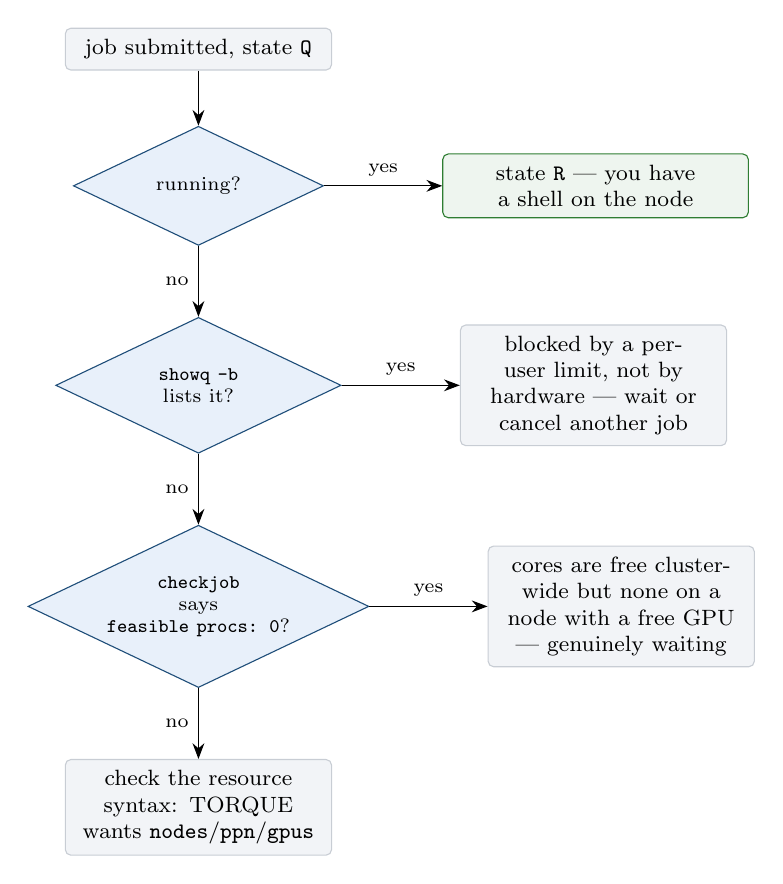
\begin{tikzpicture}[font=\footnotesize, node distance=7mm,
  box/.style={draw=rule, fill=shade, rounded corners=2pt, align=center,
              inner sep=4pt, text width=3.1cm},
  dec/.style={draw=accent, fill=laptop, diamond, aspect=2.1, align=center,
              inner sep=1pt, text width=2.5cm, font=\scriptsize},
  act/.style={draw=good, fill=good!8, rounded corners=2pt, align=center,
              inner sep=4pt, text width=3.6cm}]

\node[box] (sub) {job submitted, state \texttt{Q}};
\node[dec, below=of sub] (run) {running?};
\node[act, right=1.5cm of run] (ok) {state \texttt{R} --- you have a shell on the node};
\node[dec, below=9mm of run] (blocked) {\texttt{showq -b}\\ lists it?};
\node[box, right=1.5cm of blocked] (policy) {blocked by a per-user limit, not by hardware --- wait or cancel another job};
\node[dec, below=9mm of blocked] (feasible) {\texttt{checkjob}\\ says\\ \texttt{feasible procs: 0}?};
\node[box, right=1.5cm of feasible] (nogpu) {cores are free cluster-wide but none on a node with a free GPU --- genuinely waiting};
\node[box, below=9mm of feasible] (syntax) {check the resource syntax: TORQUE wants \texttt{nodes}/\texttt{ppn}/\texttt{gpus}};

\draw[-{Stealth[length=2mm]}] (sub) -- (run);
\draw[-{Stealth[length=2mm]}] (run) -- node[above, font=\scriptsize]{yes} (ok);
\draw[-{Stealth[length=2mm]}] (run) -- node[left, font=\scriptsize]{no} (blocked);
\draw[-{Stealth[length=2mm]}] (blocked) -- node[above, font=\scriptsize]{yes} (policy);
\draw[-{Stealth[length=2mm]}] (blocked) -- node[left, font=\scriptsize]{no} (feasible);
\draw[-{Stealth[length=2mm]}] (feasible) -- node[above, font=\scriptsize]{yes} (nogpu);
\draw[-{Stealth[length=2mm]}] (feasible) -- node[left, font=\scriptsize]{no} (syntax);
\end{tikzpicture}
\caption{Diagnosing a job that will not start. \texttt{checkjob} is the single
most useful command on the cluster; guessing is the least useful.}
\label{fig:why}
\end{figure}

\begin{lstlisting}
showq                 # EVERYONE's jobs, with time remaining
showq -i              # idle/eligible jobs, in priority order
showq -b              # blocked jobs: over a policy limit, not waiting on hardware
checkjob 67322        # why is THIS job not starting
qstat -u $USER        # my jobs only
qstat -Q              # what queues exist
qdel 67322            # cancel
\end{lstlisting}

Job states: \texttt{Q} queued, \texttt{R} running, \texttt{C} complete,
\texttt{H} held, \texttt{E} exiting.

\callout{warn}{\texttt{qstat} cannot see other users}{%
On Vega \texttt{qstat -a} shows only your own jobs, which makes the cluster look
empty when it is full. Use \textbf{\texttt{showq}} for the real picture. ``All
nodes and GPUs appear free'' in the portal is not evidence that a GPU is
available to you.}

\subsection{Nodes are shared, so a modest request gets in sooner \verified}

Jobs with 1, 8, 12, 32 and 192 cores run side by side on the same node. The
\texttt{jobs = 0-191} seen in \texttt{pbsnodes} output is one job that
\emph{asked for} all 192, not a policy of whole-node allocation. So a small
request can slot into the gap a large one leaves: measured on 5 October 2026, a
48-core single-GPU job was feasible on a node where the three higher-priority
jobs ahead of it consumed only 140 of 192 cores.

\subsection{Before you ask: which node has an idle card? \verified}
\label{sec:gpustatus}

Vega has two GPU nodes, \texttt{gpu01} and \texttt{gpu02}, with four H100s each.
Before submitting, look at both, so you can ask for the node that actually has a
free card. From the login node, SSH straight into each one. This works without
holding a job on the node:

\noindent\begin{minipage}{\linewidth}
\begin{lstlisting}
ssh gpu01 nvidia-smi --query-gpu=index,memory.used,utilization.gpu --format=csv
ssh gpu02 nvidia-smi --query-gpu=index,memory.used,utilization.gpu --format=csv
\end{lstlisting}
\end{minipage}

A card is idle when it shows near-zero memory \emph{and} 0\% utilisation, like
card~2 here:

\begin{lstlisting}
index, memory.used [MiB], utilization.gpu [%]
0, 18697 MiB, 42 %
1, 17675 MiB, 41 %
2, 0 MiB, 0 %
3, 17585 MiB, 36 %
\end{lstlisting}

Memory matters more than utilisation. A card with a model loaded and waiting
for requests shows 0\% but tens of GB in use, and it belongs to someone. To see
\emph{what} is on a busy card:

\begin{lstlisting}
ssh gpu01 nvidia-smi --query-compute-apps=gpu_uuid,pid,process_name,used_memory --format=csv
ssh gpu02 nvidia-smi --query-compute-apps=gpu_uuid,pid,process_name,used_memory --format=csv
\end{lstlisting}

\texttt{nvidia-smi} shows what the cards are doing \emph{now}. A GPU the
scheduler has just handed to another job can still look idle until that job
loads something, so if a request on a node with an idle-looking card doesn't
start, \texttt{checkjob} (Figure~\ref{fig:why}) is the next step.

\subsection{Asking for a specific node, and pointing the tunnel at it}

The plain request (\texttt{nodes=1}) lets the scheduler choose. To land on the
node with the idle card, name it:

\begin{lstlisting}
qsub -I -q gpuq -l nodes=gpu02:ppn=48:gpus=1,mem=64gb,walltime=04:00:00
\end{lstlisting}

Naming a node trades flexibility for certainty. If that node can't host the
job, it waits even though the other node is free. Check first.

\callout{accent2}{The tunnel must name the node the job is on}{%
Whichever node you get, the prompt says so (\texttt{[chikhala@gpu02 \~{}]\$})
and so does \texttt{hostname}. The tunnel in Section~\ref{sec:tunnel} names a
node explicitly, so a job on \texttt{gpu02} needs
\texttt{-L 11435:gpu02:11434}. A tunnel still pointing at \texttt{gpu01} reaches
whatever happens to be listening there: nothing, or someone else's server.

\textbf{Every new job also needs its own \texttt{ollama serve}.} The server dies
with the job that started it. Seen on 20 October 2026: a new job on
\texttt{gpu01}, the old tunnel still up, and \texttt{curl} returning
\texttt{Recv failure: Connection was reset} until the server was started inside
the new job.}

% =====================================================================
\section{Step 6 --- Which GPU is mine?}

Inside the job, this is the first thing to settle, and the documented mechanism
did not work.

\callout{accent2}{Both allocation variables were empty \verified}{%
On the allocated node, \texttt{CUDA\_VISIBLE\_DEVICES} and
\texttt{PBS\_GPUFILE} were both \textbf{empty}, so nothing told us which of the
four cards was ours. GPUs appear not to be isolated per job, which means a
careless user can disturb someone else's work.}

\callout{good}{20 October 2026: the scheduler named the card \verified}{%
Job 71111 on \texttt{gpu02} had \texttt{CUDA\_VISIBLE\_DEVICES=1} and a
\texttt{PBS\_GPUFILE} set. The card it named was idle, and the model loaded
onto it and nowhere else (71,555\,MiB on card~1). So check first, every
time, with \texttt{echo \$CUDA\_VISIBLE\_DEVICES \$PBS\_GPUFILE}. If it is set, \textbf{keep it} and skip the \texttt{export} below. If it is
empty, pick and pin a card as below. \texttt{nvidia-smi} lists all four cards
whatever the variable says. It shows which are busy, not which is yours.}

\callout{accent}{A node is not a card, and the tunnel wants the node}{%
\texttt{gpu01} is a \textbf{machine} --- the cluster has two, \texttt{gpu01} and
\texttt{gpu02}. The \texttt{2} in \texttt{CUDA\_VISIBLE\_DEVICES=2} is a
\textbf{card inside that machine}, which has four numbered 0--3. They are
unrelated numbers that both happen to be small.

It matters because the tunnel in Section~\ref{sec:tunnel} names a \emph{host and
port}. Cards are not network-addressable: the server listens on one port on
\texttt{gpu01} whichever card it uses. So the tunnel says \texttt{gpu01}
regardless --- and if the scheduler had given you \texttt{gpu02}, pointing the
tunnel at \texttt{gpu01} would reach a server someone else is running.}

The workaround, which is reading rather than guessing where possible:

\begin{lstlisting}
nvidia-smi
nvidia-smi -L
nvidia-smi --query-gpu=index,name,memory.total,memory.used,utilization.gpu --format=csv
nvidia-smi --query-compute-apps=pid,process_name,used_memory --format=csv
\end{lstlisting}

Find a card reporting near-zero memory in use, then pin to it explicitly so
nothing strays onto a neighbour's GPU:

\begin{lstlisting}
export CUDA_VISIBLE_DEVICES=0
\end{lstlisting}

\callout{warn}{This is a courtesy issue with teeth}{%
Two of \texttt{gpu01}'s four cards were idle while another job held the node.
Pinning kept our 42\,GB model off the two that were busy. A user who does not
check could silently halve someone else's throughput --- which is why this is
question one in the outstanding list for the HPC team.}

% =====================================================================
\section{Step 7 --- Serving the model, and the memory trap}
\label{sec:ctx}

\subsection{Starting the server \verified}

One command at a time, because each one answers a different question.

\textbf{Load the environment} --- this is what puts \texttt{ollama} on your
\texttt{PATH} and points it at the models in \texttt{/scratch}:

\begin{lstlisting}
source /scratch/$USER/ollama/env.sh
\end{lstlisting}

\textbf{Confirm it loaded.} A \emph{client version} is success:

\begin{lstlisting}
ollama --version
\end{lstlisting}

\callout{accent}{``could not connect to a running Ollama instance'' is expected here}{%
No server is running yet, so the client cannot reach one. What matters is that it
prints a version rather than a linker error --- a linker error means
\texttt{LD\_LIBRARY\_PATH} is wrong and the bundled CUDA libraries were not found.}

\textbf{See the four cards} and pick an idle one:

\begin{lstlisting}
nvidia-smi --query-gpu=index,memory.used,utilization.gpu --format=csv
\end{lstlisting}

A real reading from 9 October 2026 --- three cards were busy with somebody else's
job and only one was free:

\begin{lstlisting}
index, memory.used [MiB], utilization.gpu [%]
0, 18697 MiB, 42 %
1, 17675 MiB, 41 %
2, 0 MiB, 0 %
3, 17585 MiB, 36 %
\end{lstlisting}

\textbf{Pin to the free one.} Had we defaulted to 0, our 42\,GB would have landed
on top of a running job:

\begin{lstlisting}
export CUDA_VISIBLE_DEVICES=2
\end{lstlisting}

\textbf{Start the server}, which is the one command worth reading in full:

\begin{lstlisting}
OLLAMA_HOST=0.0.0.0:11434 OLLAMA_CONTEXT_LENGTH=4096 nohup ollama serve > /scratch/$USER/ollama/serve-gpu.log 2>&1 &
\end{lstlisting}

\begin{center}
\begin{tabularx}{\linewidth}{@{}>{\raggedright\arraybackslash}p{4.4cm} X@{}}
\toprule
\textbf{Fragment} & \textbf{What it does} \\
\midrule
\texttt{OLLAMA\_HOST=0.0.0.0:11434} & Binds the server to \textbf{every} network
interface rather than loopback only. This is the piece that makes the tunnel
possible: bound to \texttt{127.0.0.1} the server is invisible to the login node
and the forward is refused. \\
& Set \textbf{inline} rather than exported, so it applies to this one process.
Your own \texttt{ollama} client commands afterwards still default to
\texttt{127.0.0.1} and reach it locally. \\
\texttt{OLLAMA\_CONTEXT\_LENGTH=4096} & Caps the context window. The default is
\textbf{131{,}072}, which needs about 43\,GB of KV cache on top of 42\,GB of
weights --- 85\,GB against an 80\,GB card. See Figure~\ref{fig:kv}. \\
\texttt{nohup} & ``No hang up''. Detaches the process from this terminal's
hangup signal, so it survives if your SSH session drops. \\
\texttt{ollama serve} & The server itself. \\
\texttt{> .../serve-gpu.log} & Sends normal output to a log file.
\texttt{\$USER} expands to your username. \\
\texttt{2>\&1} & Sends \textbf{error} output (stream 2) to the same place as
normal output (stream 1), so a failure is captured rather than lost. \\
\texttt{\&} & Runs it in the background and returns your prompt. \\
\bottomrule
\end{tabularx}
\end{center}

It inherits \texttt{CUDA\_VISIBLE\_DEVICES} from the previous command, so it uses
only the card you pinned. You get a job number such as \texttt{[1] 3416817} back
--- that is the process id.

\textbf{Check the server is answering} and can see the staged models:

\begin{lstlisting}
ollama list
\end{lstlisting}

\textbf{Load the model.} The first call reads 42\,GB off Lustre, so expect
roughly 35--45 seconds before it replies:

\begin{lstlisting}
ollama run llama3.3:70b "reply with the single word: ready"
\end{lstlisting}

\textbf{And the check that actually matters:}

\begin{lstlisting}
nvidia-smi --query-gpu=index,memory.used,utilization.gpu --format=csv
\end{lstlisting}

Your card should read about \textbf{42{,}000 MiB}. A utilisation of 0\,\% is
correct for an idle server between requests --- memory is the measurement here,
not utilisation.

\subsection{Finding the server again later}

\begin{center}
\begin{tabularx}{\linewidth}{@{}l X@{}}
\toprule
\textbf{Command} & \textbf{Answers} \\
\midrule
\texttt{jobs -l} & background jobs \emph{of this shell}, with their process ids \\
\texttt{pgrep -af ollama} & every \texttt{ollama} process on the node, with its
full command line, whoever owns it \\
\texttt{nvidia-smi --query-compute-apps=pid,used\_memory --format=csv} & which
process ids are actually \textbf{on a GPU}, and how much each is using \\
\bottomrule
\end{tabularx}
\end{center}

That last one is the one worth knowing: it ties a process to GPU memory, so it
tells you whether \emph{your} server is the thing holding the 42\,GB rather than
leaving you to assume. To stop the server: \texttt{kill <pid>}, or
\texttt{pkill -f "ollama serve"}.

Binding \texttt{0.0.0.0} rather than loopback is what allows the login node to
reach the server, which is what makes the tunnel possible. Setting it inline
rather than exporting keeps your own \texttt{ollama} client commands pointed at
\texttt{127.0.0.1}.

\callout{accent}{The last \texttt{nvidia-smi} is the measurement that matters}{%
Roughly \textbf{42\,GB of VRAM in use} means the model is on the GPU. Near zero
means it quietly fell back to CPU and every timing you collect will be
meaningless.}

\subsection{Why the context length nearly ruined the experiment \verified}

This is the subtlest problem in the whole setup and worth understanding properly.

A model needs memory for two separate things: its \textbf{weights}, which are
fixed, and its \textbf{KV cache}, which scales with how many tokens it may hold
at once. Ollama's default context length for these models is \textbf{131{,}072}
tokens. On a 70B model that cache is about 43\,GB.

\begin{figure}[h]
\centering
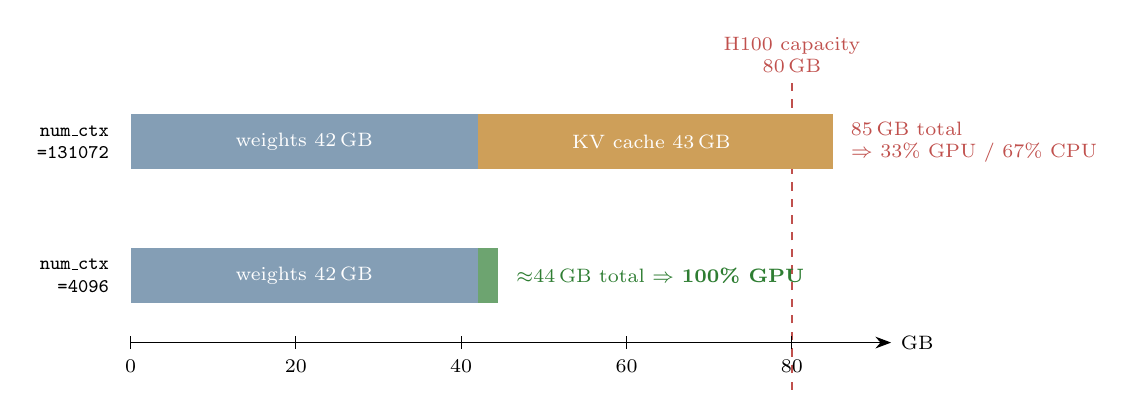
\begin{tikzpicture}[font=\footnotesize]
  \def\sc{0.105}   % cm per GB

  % -- capacity reference
  \draw[dashed, accent2, line width=0.9pt] (80*\sc,-0.4) -- (80*\sc,3.5)
    node[above, font=\scriptsize, text=accent2, align=center] {H100 capacity\\ 80\,GB};

  % -- default
  \node[left, font=\scriptsize, align=right] at (-0.15,2.75)
    {\texttt{num\_ctx}\\ \texttt{=131072}};
  \fill[accent!55] (0,2.4) rectangle (42*\sc,3.1);
  \node[font=\scriptsize, white] at (21*\sc,2.75) {weights 42\,GB};
  \fill[warn!65] (42*\sc,2.4) rectangle (85*\sc,3.1);
  \node[font=\scriptsize, white] at (63*\sc,2.75) {KV cache 43\,GB};
  \node[right, font=\scriptsize, text=accent2, align=left] at (85*\sc+0.1,2.75)
    {85\,GB total\\ $\Rightarrow$ 33\% GPU / 67\% CPU};

  % -- fixed
  \node[left, font=\scriptsize, align=right] at (-0.15,1.05)
    {\texttt{num\_ctx}\\ \texttt{=4096}};
  \fill[accent!55] (0,0.7) rectangle (42*\sc,1.4);
  \node[font=\scriptsize, white] at (21*\sc,1.05) {weights 42\,GB};
  \fill[good!70] (42*\sc,0.7) rectangle (44.5*\sc,1.4);
  \node[right, font=\scriptsize, text=good, align=left] at (44.5*\sc+0.1,1.05)
    {$\approx$44\,GB total $\Rightarrow$ \textbf{100\% GPU}};

  % -- axis
  \draw[-{Stealth[length=2mm]}] (0,0.2) -- (92*\sc,0.2);
  \foreach \g in {0,20,40,60,80} {
    \draw (\g*\sc,0.12) -- (\g*\sc,0.28);
    \node[below, font=\scriptsize] at (\g*\sc,0.1) {\g};
  }
  \node[right, font=\scriptsize] at (92*\sc,0.2) {GB};
\end{tikzpicture}
\caption{The context-length trap. Leaving \texttt{num\_ctx} at its default made
the model 5\,GB too large for the card, and Ollama responded by splitting it
67\% onto the CPU --- which is both far slower and no longer the measurement we
intended. Our planning prompts are a few hundred tokens, so 4096 is ample and
keeps the model entirely on the GPU.}
\label{fig:kv}
\end{figure}

\callout{accent}{Reducing context is not a compromise here}{%
The agent's prompts are a few hundred tokens and its replies are capped at 512.
A 4096-token window is many times what the task needs. The number to record in
the protocol is the one that was used, which is why \texttt{num\_ctx} is a
declared field in the experiment's configuration rather than a default left
implicit.}

% =====================================================================
\section{Step 8 --- The SSH tunnel}
\label{sec:tunnel}

\subsection{What a tunnel actually is}

An SSH tunnel makes a port on your laptop behave as though it were a port on a
remote machine. Traffic sent to the local port travels inside the encrypted SSH
connection, emerges at the other end, and is forwarded onward.

The important subtlety for this workflow: the forwarding happens \emph{from the
login node}. You do not need SSH access into the compute node --- you only need
the login node to be able to open an ordinary TCP connection to it, which it
can. This is what makes the whole arrangement possible without special
privileges.

\begin{figure}[h]
\centering
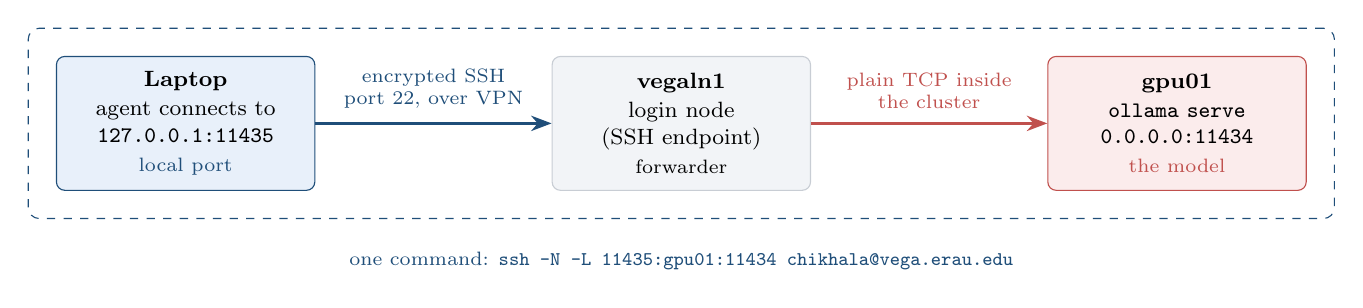
\begin{tikzpicture}[font=\footnotesize,
  m/.style={draw=rule, fill=shade, rounded corners=3pt, align=center,
            minimum height=1.7cm, text width=3.0cm, inner sep=4pt}]

% The gap between boxes has to hold a two-line label, so it is wider than the
% label rather than the other way round.
\node[m, fill=laptop, draw=accent] (lap)
  {\textbf{Laptop}\\[1pt] agent connects to\\ \texttt{127.0.0.1:11435}\\[1pt]
   \textcolor{accent}{\scriptsize local port}};
\node[m, right=3.0cm of lap] (ln)
  {\textbf{vegaln1}\\[1pt] login node\\ (SSH endpoint)\\[1pt]
   \scriptsize forwarder};
\node[m, right=3.0cm of ln, fill=cluster, draw=accent2] (gn)
  {\textbf{gpu01}\\[1pt] \texttt{ollama serve}\\ \texttt{0.0.0.0:11434}\\[1pt]
   \textcolor{accent2}{\scriptsize the model}};

% Labels sit clear above the arrows; the arrows are drawn between box borders.
\draw[-{Stealth[length=2.6mm]}, line width=1pt, accent]
  (lap.east) -- node[above=1.5pt, font=\scriptsize, align=center]
  {encrypted SSH\\ port 22, over VPN} (ln.west);
\draw[-{Stealth[length=2.6mm]}, line width=1pt, accent2]
  (ln.east) -- node[above=1.5pt, font=\scriptsize, align=center]
  {plain TCP inside\\ the cluster} (gn.west);

\begin{scope}[on background layer]
  \node[draw=accent, dashed, rounded corners=4pt,
        fit=(lap)(gn), inner sep=10pt] (frame) {};
\end{scope}

% Below the frame rather than attached to it, so it cannot land on the boxes.
\node[below=3mm of frame.south, font=\scriptsize, text=accent, align=center]
  {one command:
   \texttt{ssh -N -L 11435:gpu01:11434 chikhala@vega.erau.edu}};
\end{tikzpicture}
\caption{The three-hop path. The laptop never speaks to \texttt{gpu01}
directly; the login node relays. Note that \texttt{gpu01} must be bound to
\texttt{0.0.0.0} for the middle hop to be permitted at all.}
\label{fig:tunnel}
\end{figure}

\subsection{Opening it \verified}

From the laptop, with the VPN connected, substituting the node name you noted
from \texttt{hostname}:

\begin{lstlisting}
ssh -N -o ServerAliveInterval=30 -L 11435:gpu01:11434 chikhala@vega.erau.edu
\end{lstlisting}

\begin{center}
\begin{tabularx}{\linewidth}{@{}l X@{}}
\toprule
\textbf{Fragment} & \textbf{Meaning} \\
\midrule
\texttt{-N} & do not run a command --- forward ports only. The terminal will
appear to hang; that is correct, and it must stay open. \\
\texttt{-o ServerAliveInterval=30} & send a keepalive every 30\,s so an idle
tunnel is not dropped by a firewall \\
\texttt{-L 11435:gpu01:11434} & forward \emph{my} 11435 to \texttt{gpu01}'s
11434, resolved \emph{from the login node} \\
\bottomrule
\end{tabularx}
\end{center}

Then point the agent at it:

\begin{lstlisting}
$env:OLLAMA_HOST = "http://127.0.0.1:11435"
\end{lstlisting}

\subsection{Why 11435 and never 11434 --- a data-integrity decision}

\begin{figure}[h]
\centering
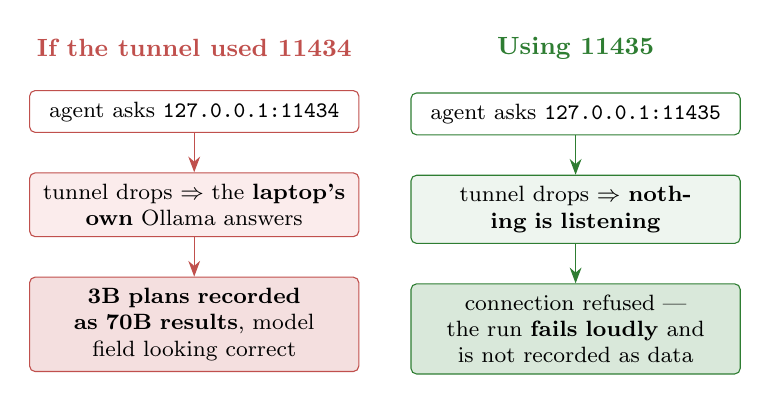
\begin{tikzpicture}[font=\footnotesize,
  m/.style={draw=rule, fill=white, rounded corners=2pt, align=center,
            inner sep=4pt, text width=3.9cm}]

% Chained with below=of rather than placed at fixed heights: these boxes hold
% two or three lines depending on the text, and a fixed spacing that fits one
% of them overlaps the others.

% -- the hazard
\node[font=\small\bfseries, text=accent2] (badt) {If the tunnel used 11434};
\node[m, draw=accent2, below=3mm of badt] (bad1)
  {agent asks \texttt{127.0.0.1:11434}};
\node[m, draw=accent2, fill=cluster, below=5mm of bad1] (bad2)
  {tunnel drops $\Rightarrow$ the \textbf{laptop's own} Ollama answers};
\node[m, draw=accent2, fill=accent2!18, below=5mm of bad2] (bad3)
  {\textbf{3B plans recorded as 70B results}, model field looking correct};

\draw[-{Stealth[length=2mm]}, accent2] (bad1) -- (bad2);
\draw[-{Stealth[length=2mm]}, accent2] (bad2) -- (bad3);

% -- the choice made
\node[font=\small\bfseries, text=good, right=1.6cm of badt] (goodt) {Using 11435};
\node[m, draw=good, below=3mm of goodt] (g1)
  {agent asks \texttt{127.0.0.1:11435}};
\node[m, draw=good, fill=good!8, below=5mm of g1] (g2)
  {tunnel drops $\Rightarrow$ \textbf{nothing is listening}};
\node[m, draw=good, fill=good!18, below=5mm of g2] (g3)
  {connection refused --- the run \textbf{fails loudly} and is not recorded as data};

\draw[-{Stealth[length=2mm]}, good] (g1) -- (g2);
\draw[-{Stealth[length=2mm]}, good] (g2) -- (g3);
\end{tikzpicture}
\caption{The port choice is not cosmetic. The laptop already runs Ollama on
11434 with \texttt{llama3.2:3b} as the control model. Reusing that port would
make a dropped tunnel \emph{silently} substitute the small model for the large
one, producing plausible, wrong, unrecoverable data. A distinct port converts
that into an immediate, obvious failure.}
\label{fig:port}
\end{figure}

This project has already lost one dataset to a measurement that looked fine and
was not. Choosing a port that fails loudly is cheaper than discovering the
substitution afterwards --- which, in general, cannot be done at all.

% =====================================================================
\section{Step 9 --- Wiring the agent, and refusing to fly blind}

A tunnel that works is not sufficient. The record has to \emph{prove} which
model produced each plan, so three changes were made to the agent.

\subsection{The endpoint is explicit and recorded}

\begin{lstlisting}
OLLAMA_ENDPOINT = os.environ.get("OLLAMA_HOST") or "http://127.0.0.1:11434"
\end{lstlisting}

It is accepted either as \texttt{host:port} or as a full URL, normalised once,
and written into every planning record and the provenance manifest. A result
that cannot say where it came from is not evidence.

\subsection{A pre-flight check that refuses to proceed}

Before any aircraft is armed, the agent asks the endpoint which models it serves
and requires an exact match for the one the protocol declares:

\begin{lstlisting}
curl -s http://127.0.0.1:11435/api/tags
\end{lstlisting}

If the endpoint is unreachable, or reachable but serving a different model, the
run is refused with a message that mentions the tunnel. The alternative --- 30
missions flown against the wrong model --- is a wasted session at best.

\subsection{Transport failures are not model failures}

A dropped VPN must not be recorded as the model producing an invalid plan.
Exceptions are classified by origin, so a network failure is marked
\texttt{transport\_error} and \textbf{excluded from both the numerator and the
denominator} of the correctness score. Otherwise a flaky connection would look
like a less capable model.

\subsection{Inference options are declared, not defaulted}

\begin{center}
\begin{tabularx}{\linewidth}{@{}l l X@{}}
\toprule
\textbf{Option} & \textbf{Value} & \textbf{Why it is recorded} \\
\midrule
\texttt{num\_gpu} & 999 & all layers on the GPU. The laptop forces \texttt{0}
because its VRAM belongs to the simulator; the data must say which \\
\texttt{num\_ctx} & 4096 & see Figure~\ref{fig:kv} --- the default would move
67\% of the model to the CPU \\
\texttt{temperature} & 0 & deterministic output, so repeats are repeats \\
\texttt{num\_predict} & 512 & a plan is short; this bounds a runaway reply \\
\bottomrule
\end{tabularx}
\end{center}

% =====================================================================
\section{Step 10 --- Proving it works, in order}

Each rung tests one thing, so a failure localises itself.

\begin{center}
\begin{tabularx}{\linewidth}{@{}c >{\raggedright\arraybackslash}p{5.0cm} X@{}}
\toprule
\textbf{\#} & \textbf{Check} & \textbf{Passes when} \\
\midrule
1 & \texttt{Test-NetConnection vega.erau.edu -Port 22} & \texttt{TcpTestSucceeded : True} \\
2 & \texttt{ssh chikhala@vega.erau.edu} & a prompt on \texttt{vegaln1} \\
3 & \texttt{qstat -u \$USER} inside the job & state \texttt{R} \\
4 & \texttt{nvidia-smi} on the node & a card with free memory \\
5 & \texttt{nvidia-smi} after loading & $\approx$\textbf{42\,GB} in use \\
6 & \texttt{curl 127.0.0.1:11435/api/tags} from the laptop & JSON listing \texttt{llama3.3:70b} \\
7 & the agent's pre-flight check & ``endpoint serving \texttt{llama3.3:70b}'' \\
8 & one mission, \texttt{--plan-only} & a valid plan, no simulator needed \\
9 & one mission, flown & plan correct \emph{and} the aircraft lands \\
10 & the control model & Vega's 3B matches the laptop's 3B plan for plan \\
\bottomrule
\end{tabularx}
\end{center}

\subsection{What the working system looked like \verified}

\begin{center}
\begin{tabularx}{\linewidth}{@{}l X@{}}
\toprule
Model & \texttt{llama3.3:70b}, 4-bit, 42\,GB \\
Placement & \textbf{100\% GPU} on one H100 80\,GB \\
Host & Vega, node \texttt{gpu01}, 4\,h walltime. Job \textbf{67322} via
\texttt{batch} on 6 October; job \textbf{67630} via \texttt{gpuq} on 9 October,
after the queue split --- see Section~\ref{sec:queues} \\
Reached by & SSH tunnel through \texttt{vegaln1}, laptop port 11435 \\
Simulator & local --- CarlaAir v0.1.7, Town10HD, Epic quality, traffic on \\
Round trip & $\approx$3.7\,s for a cold \texttt{/api/tags}; 0.1\,s once warm \\
Planning latency & \textbf{34.9\,s} on the first call (loading 42\,GB), then
\textbf{0.7--1.8\,s} \\
Delivered & 30 missions, 42 planning calls, every one answered \\
\bottomrule
\end{tabularx}
\end{center}

\callout{good}{The result worth knowing}{%
\texttt{llama3.2:3b} on this laptop's CPU plans in 1.2--1.3\,s. The 70B on an
H100 plans in \textbf{0.7--1.8\,s} --- roughly \emph{twice as fast} despite being
twenty-three times larger, because the work moved off laptop cores that the
simulator also needs. In this architecture there is no latency penalty for the
larger model.}


% =====================================================================
\section{Step 11 --- Running the experiment, from the laptop}

Everything so far was setup. This is the command that produces data.

\subsection{Three things the laptop needs first}

\subsubsection{The conda environment}

\begin{lstlisting}
conda activate carlaAir
\end{lstlisting}

\callout{accent2}{A fresh terminal does NOT have it}{%
Opening a new PowerShell gives you Miniconda's \textbf{base} interpreter, which
has no \texttt{airsim} and no \texttt{ollama} package, and the run dies on
\texttt{ModuleNotFoundError: No module named 'airsim'}. Nothing is activated by
default --- \texttt{\$env:CONDA\_DEFAULT\_ENV} is empty in a new window. You can
tell it worked because the prompt gains a \texttt{(carlaAir)} prefix.}

To skip activation entirely, name the interpreter directly --- this works in any
window:

\begin{lstlisting}
& "<miniconda>\envs\carlaAir\python.exe" scripts\run_missions.py ...
\end{lstlisting}

\subsubsection{The simulator}

\begin{lstlisting}
cd $env:CARLAAIR_ROOT
.\CarlaAir.ps1 Town10HD
\end{lstlisting}

\texttt{\$env:CARLAAIR\_ROOT} is PowerShell's syntax for reading an environment
variable, set once in \texttt{SETUP.md} so no document has to name one machine's
drive letter. If it is not set, \texttt{cd} silently does nothing --- check with
\texttt{echo \$env:CARLAAIR\_ROOT} before blaming anything else.

\subsubsection{The tunnel}

Open, and left open, in its own window. Section~\ref{sec:tunnel}.

\subsection{The command}

\begin{lstlisting}
cd "<repository root>"; python scripts\run_missions.py --missions M01,M02,M03,M04,M05,M06,M07,M08 --block v4-polled --ollama-host http://127.0.0.1:11435
\end{lstlisting}

\begin{center}
\begin{tabularx}{\linewidth}{@{}>{\raggedright\arraybackslash}p{5.2cm} X@{}}
\toprule
\textbf{Fragment} & \textbf{What it does} \\
\midrule
\texttt{cd "..."} & The working directory \textbf{matters}. The runner resolves
the mission config, the results folder and the agent relative to the repository,
so running it from elsewhere finds the wrong files or none. Quoted because the
repository folder's name contains a space. \\
\texttt{;} & PowerShell's statement separator --- run the second command after
the first, regardless of whether it succeeded. (PowerShell~5.1 has no
\texttt{\&\&}.) \\
\texttt{python} & Must be the \texttt{carlaAir} interpreter. See above. \\
\texttt{scripts{\textbackslash}run\_missions.py} & The experiment entry point.
\texttt{scripts/} produces evidence; \texttt{tools/} never appears in a result. \\
\texttt{-{}-missions M01,...,M08} & Comma-separated mission ids, matching the
\texttt{[[mission]]} entries in
\texttt{configs/missions/baseline\_v1.toml}. Omit it and every mission in the
config runs. \\
\texttt{-{}-block v4-polled} & A short label for this session. It appears in
every filename written, so the results folder reads as a list of named sessions
rather than bare timestamps. Purely organisational --- it changes nothing about
the flight. \\
\texttt{-{}-ollama-host}\newline\texttt{http://127.0.0.1:11435} & \textbf{The endpoint.} Port
11435 is the local end of the SSH tunnel, so this is what sends planning to the
70B on Vega. It is recorded in every planning record and in the provenance
manifest, so the data can say where each plan came from. \\
\bottomrule
\end{tabularx}
\end{center}

\subsubsection{Flags not used here, and when they matter}

\begin{center}
\begin{tabularx}{\linewidth}{@{}>{\raggedright\arraybackslash}p{5.2cm} X@{}}
\toprule
\texttt{-{}-plan-only} & Plan and score \textbf{without flying}. Needs no
simulator at all, so it is the fast way to check the model end of the pipeline. \\
\texttt{-{}-repeats N} & Override the protocol's repeat count. The protocol says
3, which is where ``30 runs'' comes from: 10 missions $\times$ 3. \\
\texttt{-{}-model NAME} & Override the config's model, e.g. to run the
\texttt{llama3.2:3b} control against the same set. \\
\texttt{-{}-option KEY=VALUE} & Override one inference option, repeatable ---
e.g. \texttt{-{}-option num\_gpu=999}. Whatever is used is recorded. The laptop
needs \texttt{num\_gpu=0} because the simulator owns its VRAM; a GPU server does
not. \\
\texttt{-{}-pause} & Wait for a keypress between runs, for watching each one. \\
\texttt{-{}-config} / \texttt{-{}-out} & Point at a different mission set or
results folder. Rarely needed. \\
\bottomrule
\end{tabularx}
\end{center}

\subsection{What it then does, in order}

\begin{enumerate}
  \item Reads the mission config and the \texttt{[protocol]} block --- model,
        repeats, map, quality, traffic, inference options.
  \item \textbf{Checks the endpoint before anything else}: asks what models it
        serves and requires an exact match for the one the protocol declares. A
        dead tunnel stops the run here rather than 30 missions later.
  \item Writes \texttt{settings.json} for the roster the missions need, and
        snapshots the code that is about to fly into the results folder.
  \item For each mission, for each repeat: resets the world, asks the model for
        one plan per drone, validates each against the schema, then flies them
        concurrently through \texttt{fly\_plans} with the separation and
        collision monitor running.
  \item Writes a JSONL file --- one line per run, holding the plan, the raw
        model output, the latency, the flight outcome, the altitude reached
        after every step, and the provenance --- plus a Markdown summary table.
\end{enumerate}

\callout{accent}{Where the output goes, and why there are two places}{%
\texttt{phases/phase-01-baseline-freeze/results/} holds the curated, tracked
evidence for one scored series. \texttt{runs/agent-log.jsonl} is a separate,
git-ignored log of \emph{every} planning call ever made on the machine, whatever
invoked it. The first is the experimental record; the second is a black box
recorder. Neither replaces the other.}

\subsection{Expected timings}

\begin{center}
\begin{tabularx}{\linewidth}{@{}l X@{}}
\toprule
First planning call & \textbf{35--47\,s} --- loading 42\,GB off Lustre, once per
session \\
Every call after & \textbf{0.7--2.8\,s}, depending on plan length \\
One single-drone run & about a minute, planning and flight together \\
24 runs (M01--M08) & roughly 15 minutes \\
\bottomrule
\end{tabularx}
\end{center}

\callout{warn}{Run the multi-drone missions as their own block}{%
The runner spawns the whole roster at the start of a block. Run all ten missions
together and the single-drone missions fly with four drones sitting on the pad
--- different conditions from a 24-run block, and not comparable with it. Fly
\texttt{M01--M08}, then \texttt{M09}, then \texttt{M10}, as three commands.}

% =====================================================================
\section{Step 12 --- The interactive session}

\subsection{The idea}

A benchmark answers the questions you thought of in advance. Ten missions, three
repeats, a score. What it cannot tell you is what happens at the edges of the
plan language --- what the model does with a phrasing nobody anticipated, or an
instruction the eight available actions cannot express.

\begin{lstlisting}
python tools\fly_chat.py
\end{lstlisting}

So this is a \textbf{sandbox}: ask for any number of drones at any speed, type an
instruction in plain English, look at the plan the model produced, and decide
whether to fly it. Nothing is scored and nothing is recorded.

\callout{accent}{Why it has to share the study's code path}{%
A tool that flew missions \emph{differently} from the runner would teach you
things that are not true of the experiment. So \texttt{fly\_chat.py} does not
implement flight: it calls \texttt{plan\_for} and \texttt{fly\_plans}, the same
functions the runner uses, and inherits the same system prompt, schema,
validator, inference options, thread model, ground barrier and separation
monitor. The agent's own comment on \texttt{fly\_plans} says this outright ---
shared \emph{on purpose}, because otherwise ``scored runs and hand-flown runs
would not be the same experiment, and nobody would notice until the numbers
disagreed''.}

\begin{figure}[htbp]
\centering
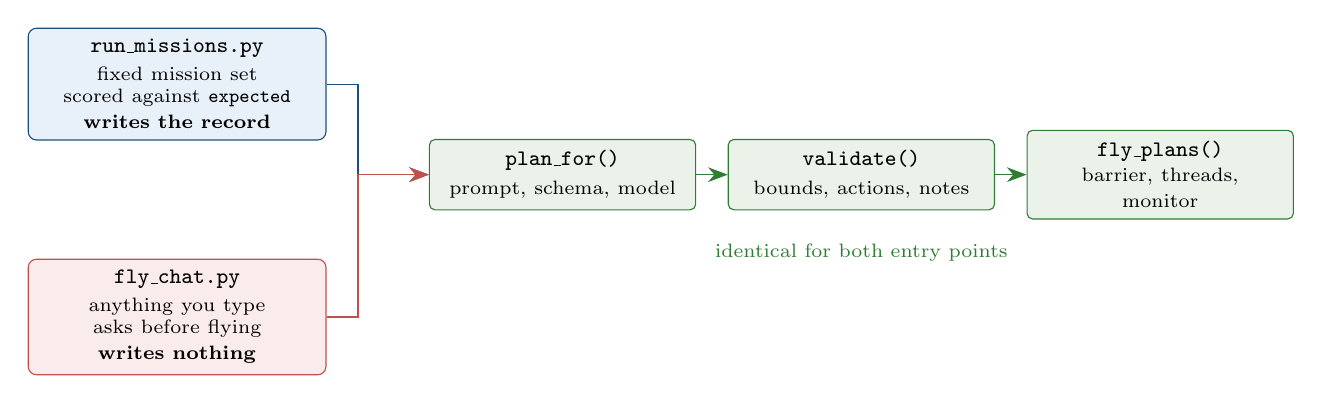
\begin{tikzpicture}[font=\footnotesize,
  entry/.style={draw=accent, fill=laptop, rounded corners=3pt, align=center,
                text width=3.5cm, inner sep=4pt},
  shared/.style={draw=good, fill=good!10, rounded corners=2pt, align=center,
                 text width=3.1cm, inner sep=4pt},
  out/.style={draw=rule, fill=shade, rounded corners=2pt, align=center,
              text width=3.3cm, inner sep=5pt}]

\node[entry] (runner)
  {\texttt{run\_missions.py}\\[2pt]
   \scriptsize fixed mission set\\ \scriptsize scored against \texttt{expected}\\
   \scriptsize \textbf{writes the record}};
\node[entry, below=1.5cm of runner, draw=accent2, fill=cluster] (chat)
  {\texttt{fly\_chat.py}\\[2pt]
   \scriptsize anything you type\\ \scriptsize asks before flying\\
   \scriptsize \textbf{writes nothing}};

\node[shared, right=1.3cm of runner, yshift=-1.15cm] (plan) {\texttt{plan\_for()}\\[1pt] \scriptsize prompt, schema, model};
\node[shared, right=4mm of plan] (val) {\texttt{validate()}\\[1pt] \scriptsize bounds, actions, notes};
\node[shared, right=4mm of val] (fly) {\texttt{fly\_plans()}\\[1pt] \scriptsize barrier, threads,\\ \scriptsize monitor};

\draw[-{Stealth[length=2.5mm]}, accent] (runner.east) -- ++(0.4,0) |- (plan.west);
\draw[-{Stealth[length=2.5mm]}, accent2] (chat.east) -- ++(0.4,0) |- (plan.west);
\draw[-{Stealth[length=2.5mm]}, good] (plan) -- (val);
\draw[-{Stealth[length=2.5mm]}, good] (val) -- (fly);

\node[font=\scriptsize, text=good, below=3mm of val, align=center]
  {identical for both entry points};
\end{tikzpicture}
\caption{Two entry points, one flight path. The differences are confined to what
goes in (a fixed set versus whatever you type) and what comes out (a scored
record versus nothing at all). Everything between them is shared, which is what
makes an observation in the sandbox worth anything.}
\label{fig:sharedpath}
\end{figure}

\subsection{What a session looks like}

Figure~\ref{fig:chatloop} is the whole loop. Every path returns to the
prompt, and the only route to the aircraft moving is an explicit \texttt{y}.

\begin{figure}[p]
\centering
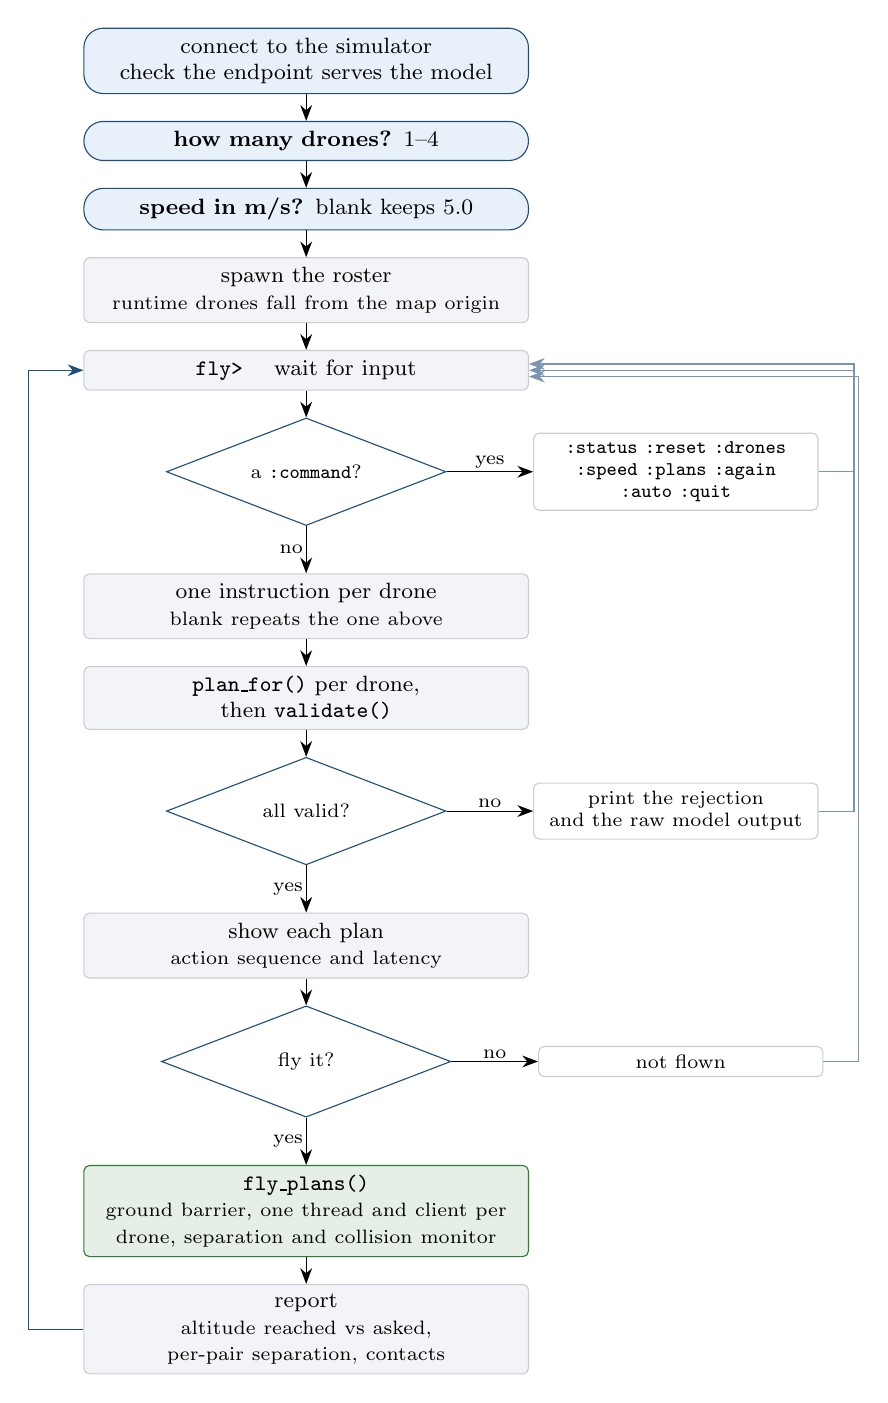
\begin{tikzpicture}[font=\footnotesize, node distance=3.4mm,
  io/.style={draw=accent, fill=laptop, rounded corners=7pt, align=center,
             text width=5.4cm, inner sep=3.5pt},
  proc/.style={draw=rule, fill=shade, rounded corners=2pt, align=center,
               text width=5.4cm, inner sep=3.5pt},
  flyb/.style={draw=good, fill=good!12, rounded corners=2pt, align=center,
               text width=5.4cm, inner sep=3.5pt},
  dec/.style={draw=accent, fill=white, align=center, text width=2.6cm,
              inner sep=2pt, font=\scriptsize, diamond, aspect=2.6},
  side/.style={draw=rule, fill=white, rounded corners=2pt, align=center,
               text width=3.4cm, inner sep=3pt, font=\scriptsize},
  lbl/.style={font=\scriptsize, inner sep=1pt}]

\node[io] (start) {connect to the simulator\\ check the endpoint serves the model};
\node[io, below=of start] (nd) {\textbf{how many drones?} 1--4};
\node[io, below=of nd] (sp) {\textbf{speed in m/s?} blank keeps 5.0};
\node[proc, below=of sp] (spawn) {spawn the roster\\ \scriptsize runtime drones fall from the map origin};
\node[proc, below=of spawn] (prompt) {\texttt{fly>} \quad wait for input};
\node[dec, below=of prompt] (iscmd) {a \texttt{:command}?};
\node[proc, below=6mm of iscmd] (instr) {one instruction per drone\\ \scriptsize blank repeats the one above};
\node[proc, below=of instr] (planning) {\texttt{plan\_for()} per drone,\\ then \texttt{validate()}};
\node[dec, below=of planning] (valid) {all valid?};
\node[proc, below=6mm of valid] (show) {show each plan\\ \scriptsize action sequence and latency};
\node[dec, below=of show] (conf) {fly it?};
\node[flyb, below=6mm of conf] (flyn) {\texttt{fly\_plans()}\\ \scriptsize ground barrier, one thread and client per drone, separation and collision monitor};
\node[proc, below=of flyn] (rep) {report\\ \scriptsize altitude reached vs asked, per-pair separation, contacts};

\node[side, right=1.1cm of iscmd] (cmd)
  {\texttt{:status :reset :drones}\\ \texttt{:speed :plans :again}\\ \texttt{:auto :quit}};
\node[side, right=1.1cm of valid] (rej)
  {print the rejection\\ and the raw model output};
\node[side, right=1.1cm of conf] (no) {not flown};

\foreach \a/\b in {start/nd, nd/sp, sp/spawn, spawn/prompt, prompt/iscmd,
                   instr/planning, planning/valid, show/conf, flyn/rep}
  \draw[-{Stealth[length=2mm]}] (\a) -- (\b);

\draw[-{Stealth[length=2mm]}] (iscmd) -- node[lbl, left]{no} (instr);
\draw[-{Stealth[length=2mm]}] (valid) -- node[lbl, left]{yes} (show);
\draw[-{Stealth[length=2mm]}] (conf) -- node[lbl, left]{yes} (flyn);

\draw[-{Stealth[length=2mm]}] (iscmd) -- node[lbl, above]{yes} (cmd);
\draw[-{Stealth[length=2mm]}] (valid) -- node[lbl, above]{no} (rej);
\draw[-{Stealth[length=2mm]}] (conf) -- node[lbl, above]{no} (no);

% everything returns to the prompt
\draw[-{Stealth[length=2mm]}, accent]
  (rep.west) -- ++(-0.7,0) |- (prompt.west);
\draw[-{Stealth[length=2mm]}, accent!60]
  (cmd.east) -- ++(0.45,0) |- ($(prompt.east)+(0,0.08)$);
\draw[-{Stealth[length=2mm]}, accent!60]
  (rej.east) -- ++(0.45,0) |- ($(prompt.east)+(0,0.0)$);
\draw[-{Stealth[length=2mm]}, accent!60]
  (no.east) -- ++(0.45,0) |- ($(prompt.east)-(0,0.08)$);
\end{tikzpicture}
\caption{The session loop. Every path returns to the prompt, and the only route
to the aircraft moving is an explicit \texttt{y}. A rejected plan prints the raw
model output rather than failing silently, because what the model emitted is
usually the interesting part.}
\label{fig:chatloop}
\end{figure}

\subsection{The details that matter}

\begin{center}
\begin{tabularx}{\linewidth}{@{}>{\raggedright\arraybackslash}p{3.5cm} X@{}}
\toprule
\textbf{Drone count} & Asked once at the start, changeable with
\texttt{:drones N}. More than one spawns them into the running simulator
immediately, not at flight time. \\
\textbf{Speed} & Asked once, changeable with \texttt{:speed N}. It also
\textbf{rewrites the system prompt}, because the speed is baked into it when the
module loads --- without that the aircraft flies at one speed while the model
reasons about another, and every duration it chooses is wrong. \\
\textbf{Confirmation} & On by default. \texttt{:auto} turns it off. \\
\textbf{Recording} & None. \texttt{plan\_for} and \texttt{fly\_plans} do not
log; only the runner's \texttt{main()} does. So no results file and no entry in
\texttt{runs/agent-log.jsonl}. \\
\textbf{Recovery} & \texttt{:reset} returns every drone to its start pose. That
is the exit from a stranded or wedged aircraft. \\
\bottomrule
\end{tabularx}
\end{center}

\callout{warn}{What it cannot do, and why that is the agent's limit not the tool's}{%
Eight actions and no yaw, so no circling, orbiting, following or searching ---
and ``turn left'' can only become a sideways strafe. No camera and no sensing:
the model plans before takeoff and is never consulted again, so ``find the red
car'' or ``stop at the wall'' are outside the architecture, not merely the
vocabulary. The drones are not told about each other, so ``follow Drone1''
cannot work. And there is \textbf{no collision avoidance anywhere in the stack}.
All of that is the frozen Phase~1 baseline; the sandbox simply lets you watch it
honestly.}

\begin{center}
\begin{tabularx}{\linewidth}{@{}l X@{}}
\toprule
\texttt{:status} & where every drone is \\
\texttt{:reset} & return all drones to their start poses --- the recovery \\
\texttt{:drones N} & change the roster mid-session \\
\texttt{:speed N} & change speed, \emph{and} tell the model about it \\
\texttt{:plans} & the raw JSON the model returned \\
\texttt{:again} & re-fly the last plans without asking the model \\
\texttt{:auto} & stop asking for confirmation \\
\bottomrule
\end{tabularx}
\end{center}

\subsection{Two findings it produced on its first use}

Both from one instruction --- \emph{fly in circles clockwise with a diameter of
30 metres, three times, then land where you took off}.

\textbf{The model treats \texttt{fly\_right} as a turn. It is a strafe.} The 70B
built the circle as \texttt{fly\_straight} $\rightarrow$ \texttt{fly\_right},
repeated --- which closes a loop only if the aircraft's heading changes. Nothing
in this agent yaws, so forward is always the same world direction and the plan
flew a diagonal staircase about 225\,m out. The model's reasoning was sound for
the action \emph{names} it was given; the names do not match the semantics.

\textbf{An unbounded \texttt{fly\_to} is a hard hang.} The return leg met a
hotel. \texttt{moveToPositionAsync} had no timeout, so the drone pushed into the
building indefinitely, holding its worker thread, which held the main thread ---
and \texttt{Ctrl-C} could not be delivered into a blocked RPC call. The only exit
was killing the simulator. Now bounded, the same way \texttt{land} is.

\callout{warn}{There is no collision avoidance anywhere in this stack}{%
Vertical staggering and spawn spacing are the only separation there is. A plan
that flies 200\,m across a city will meet a building, and the aircraft will not
avoid it. Fly above the skyline, or slow down with \texttt{:speed 1} so every
distance shrinks fivefold.}

% =====================================================================
\section{Troubleshooting}

\begin{center}
\begin{tabularx}{\linewidth}{@{}>{\raggedright\arraybackslash}p{4.6cm} X@{}}
\toprule
\textbf{Symptom} & \textbf{Cause and remedy} \\
\midrule
\texttt{Unknown queue MSG=requested queue not found} & That queue does not exist.
\texttt{qstat -Q} lists the real ones. \\
\texttt{Queue is not enabled MSG=queue is disabled} & The queue exists but is
closed to new jobs. \texttt{batch} went this way on 9 October when \texttt{gpuq}
went live. Check the \texttt{Ena} column of \texttt{qstat -Q}. \\
\texttt{ModuleNotFoundError: No module named 'airsim'} & The conda environment is
not active. \texttt{conda activate carlaAir}, or name the interpreter in full. \\
\texttt{cd \$env:CARLAAIR\_ROOT} does nothing & The variable is not set in
\emph{this} window. \texttt{setx} only affects new sessions. Check with
\texttt{echo \$env:CARLAAIR\_ROOT}. \\
A drone wedges against a building and the run will not stop & Contact with
anything can stall a flight call. \texttt{Ctrl-C} cannot interrupt a blocked RPC
call, so kill the simulator: \texttt{Stop-Process -Name
CarlaUE4,CarlaUE4-Win64-Shipping -Force}. \\
Job queues forever, no error & Almost always TORQUE syntax. Use
\texttt{nodes}/\texttt{ppn}/\texttt{gpus}; \texttt{select}/\texttt{ncpus}/\texttt{ngpus}
are accepted and never satisfied. Confirm with \texttt{checkjob}. \\
\texttt{checkjob} says \texttt{feasible procs: 0} & Cores are free cluster-wide
but none on a node with an available GPU. Genuinely waiting, not misconfigured. \\
Portal GPU session never starts & The portal submits GPU sessions to
\texttt{normalq}, which is being restricted to CPU nodes, making the request
unsatisfiable \emph{with no error shown}. Submit from the terminal instead. \\
Cluster looks empty but nothing runs & \texttt{qstat} shows only your jobs. Use
\texttt{showq}. \\
\texttt{nvidia-smi} shows near-zero memory & The model fell back to CPU. Check
\texttt{num\_gpu}, and check \texttt{num\_ctx} (Figure~\ref{fig:kv}). \\
Model loads at 33\% GPU / 67\% CPU & The KV cache made it exceed 80\,GB. Set
\texttt{OLLAMA\_CONTEXT\_LENGTH=4096}. \\
\texttt{curl} on 11435 refuses & The tunnel is down, or the server was bound to
loopback instead of \texttt{0.0.0.0}, or the job's walltime expired. \\
Tunnel listening, nothing answers & The job ended. The forwarder survives the
job, so \texttt{netstat} still shows a listener --- check \texttt{qstat -u
\$USER}. \\
\texttt{curl: (56) Recv failure: Connection was reset} on 11435 & The tunnel
and SSH hop work, but nothing is listening on \texttt{<node>:11434}. Either the
new job has no \texttt{ollama serve} yet (start it, Step~7), or the job is on
the other node and the tunnel still names the old one
(Section~\ref{sec:gpustatus}). Seen 20 October 2026. \\
\texttt{ollama --version} gives a linker error after an update & The new
\texttt{lib/} did not extract cleanly. Extract again, or reinstall a release by
its tag (Section~\ref{sec:update}). \\
\texttt{sha256sum: ... no file was verified} & The archive was saved under a
different name from the one in the checksum file. Look the hash up with
\texttt{grep} instead (Section~\ref{sec:update}, Step~4). Seen 19 October 2026. \\
\texttt{ollama list} fails on the login node & From 0.40.6 it needs a running
server. Read \texttt{models/manifests/registry.ollama.ai/library} instead. \\Downloaded archive is 9 bytes & The documented Ollama URL 404s. Use the
\texttt{.tar.zst} asset and check the size. \\
\texttt{tar: unrecognized option --zstd} & Rocky 8's tar is too old. Pipe:
\texttt{zstd -dc file.tar.zst | tar -xf -} \\
\texttt{could not connect to a running Ollama instance} & Expected with no
server running. A \emph{linker} error instead means
\texttt{LD\_LIBRARY\_PATH} is wrong. \\
\texttt{CUDA\_VISIBLE\_DEVICES} empty & Not populated on this cluster. Read
\texttt{nvidia-smi}, pick an idle card, pin it explicitly. \\
\bottomrule
\end{tabularx}
\end{center}

% =====================================================================
\section{Shutting down properly}

Eight GPUs serve the whole university, so holding an idle one is a policy matter
rather than a courtesy.

\begin{lstlisting}
pkill -f "ollama serve"     # on the GPU node
exit                        # ends the interactive job, releasing the GPU
qstat -u $USER              # confirm nothing of yours is still running
pgrep -af ollama            # confirm no stray server
\end{lstlisting}

Then close the SSH tunnel window on the laptop. Verify from the laptop that
nothing is still held:

\begin{lstlisting}
ssh chikhala@vega.erau.edu "qstat -u $USER; pgrep -af ollama"
\end{lstlisting}

\callout{warn}{An interactive job's walltime runs from when it starts, not when you arrive}{%
If a queued interactive job begins overnight, it holds a GPU doing nothing until
the walltime expires. Ask for a window you will actually be present for, and
cancel and resubmit rather than letting one idle.}

% =====================================================================
\section{Open questions}

Recorded because an unanswered question is part of the state of the work.

\begin{enumerate}
  \item \textbf{How should a job read its GPU allocation?} Both
        \texttt{CUDA\_VISIBLE\_DEVICES} and \texttt{PBS\_GPUFILE} were empty.
        Reading \texttt{nvidia-smi} and pinning works but relies on guessing
        correctly, and guessing wrong disturbs another user's job.
  \item \textbf{Does \texttt{/scratch} get purged?} 47\,GB of weights live
        there and it is unclear whether they must be re-staged.
  \item \textbf{Is there a shared model cache?} Several users downloading the
        same 42\,GB model separately wastes a great deal of space.
  \item \textbf{Is a long-running inference server inside a job, reached by SSH
        forwarding, a supported pattern?} It works cleanly; confirmation is
        better than assumption.
  \item \textbf{Is there a reservation mechanism for interactive work?} See the
        walltime warning above.
  \item \textbf{\sout{When will \texttt{gpuq} exist?}} \textbf{Answered
        9 October 2026}: it exists, it works, and a request that waited two
        hours before the split now starts immediately. \texttt{batch} was
        disabled in the same change. Kept here because the sequence is the
        lesson --- the restriction half of a change can land before the half
        that makes it usable, and for three days there was no documented route
        to a GPU at all.
\end{enumerate}

% =====================================================================
\appendix
\section{Command reference}

\subsection{Laptop, before anything else}
\begin{lstlisting}
Test-NetConnection vega.erau.edu -Port 22
\end{lstlisting}

\subsection{On the login node}
\begin{lstlisting}
ssh chikhala@vega.erau.edu
hostname; echo $0; pwd; echo $HOME; echo $USER
df -h ~ /scratch
du -sh /scratch/$USER
source /scratch/$USER/ollama/env.sh
ollama --version
ollama list
\end{lstlisting}

\subsection{Seeing the cluster}
\begin{lstlisting}
showq                       # everyone's jobs
showq -i                    # idle, in priority order
showq -b                    # blocked by policy
checkjob <jobid>            # why is this job not starting
qstat -u $USER
qstat -Q
qstat -f <jobid>
qdel <jobid>

pbsnodes -a | awk '/^[^ ]/{n=$1} /^ *state =/{print n, $3}'
pbsnodes -a | awk '/^ *state =/{print $3}' | sort | uniq -c
pbsnodes gpu01 gpu02 | grep -E "^gpu|state =|jobs ="
pbsnodes gpu01 | tr ',' '\n' | grep -E "ncpus|loadave|totmem|availmem"
\end{lstlisting}

\subsection{Which cards are idle, on both GPU nodes}
\begin{lstlisting}
ssh gpu01 nvidia-smi --query-gpu=index,memory.used,utilization.gpu --format=csv
ssh gpu02 nvidia-smi --query-gpu=index,memory.used,utilization.gpu --format=csv

ssh gpu01 nvidia-smi --query-compute-apps=gpu_uuid,pid,process_name,used_memory --format=csv
ssh gpu02 nvidia-smi --query-compute-apps=gpu_uuid,pid,process_name,used_memory --format=csv
\end{lstlisting}

\subsection{Getting a GPU}
\begin{lstlisting}
qstat -Q                    # which queues exist, and is Ena = yes
qsub -I -q gpuq -l nodes=1:ppn=48:gpus=1,mem=64gb,walltime=04:00:00
qsub -I -q gpuq -l nodes=gpu02:ppn=48:gpus=1,mem=64gb,walltime=04:00:00   # a named node
hostname                    # which node you got -- the tunnel must name it
\end{lstlisting}

\subsection{Updating Ollama (login node, nothing serving)}
\begin{lstlisting}
source /scratch/$USER/ollama/env.sh
ollama --version
pgrep -af "ollama serve"                 # must print nothing
curl -s https://api.github.com/repos/ollama/ollama/releases/latest | grep '"tag_name"'

cd /scratch/$USER/ollama
curl -L --progress-bar -o ollama-0.40.6.tar.zst \
  https://github.com/ollama/ollama/releases/download/v0.40.6/ollama-linux-amd64.tar.zst
ls -lh ollama-0.40.6.tar.zst        # ~1.44 GB
curl -sL -o sha256sum-0.40.6.txt \
  https://github.com/ollama/ollama/releases/download/v0.40.6/sha256sum.txt
grep -F "$(sha256sum ollama-0.40.6.tar.zst | cut -d' ' -f1)" sha256sum-0.40.6.txt && echo VERIFIED

rm -rf bin lib                           # only after VERIFIED
zstd -dc ollama-0.40.6.tar.zst | tar -xf -
ollama --version && ls lib/ollama | grep -i cuda
du -sh models && ls models/manifests/registry.ollama.ai/library
rm -f ollama-0.40.6.tar.zst
\end{lstlisting}

\subsection{On the GPU node}
\begin{lstlisting}
source /scratch/$USER/ollama/env.sh
hostname
nvidia-smi
echo "CUDA_VISIBLE_DEVICES=[$CUDA_VISIBLE_DEVICES]"   # set by the scheduler? keep it
export CUDA_VISIBLE_DEVICES=0                       # only if it was empty

OLLAMA_HOST=0.0.0.0:11434 OLLAMA_CONTEXT_LENGTH=98304 \
  nohup ollama serve > /scratch/$USER/ollama/serve-gpu.log 2>&1 &

ollama run llama3.3:70b "reply with the single word: ready"
nvidia-smi
\end{lstlisting}

\subsection{From the laptop}
\begin{lstlisting}
ssh -N -o ServerAliveInterval=30 -L 11435:gpu01:11434 chikhala@vega.erau.edu
# job on gpu02?  then:  -L 11435:gpu02:11434
\end{lstlisting}

\begin{lstlisting}
curl -s http://127.0.0.1:11435/api/tags
curl -s http://127.0.0.1:11435/api/version    # the version the runner will record
\end{lstlisting}

\begin{lstlisting}
conda activate carlaAir
cd $env:CARLAAIR_ROOT
.\CarlaAir.ps1 Town10HD
\end{lstlisting}

\begin{lstlisting}
cd "<repository root>"
python scripts\run_missions.py --missions M01 --repeats 1 --ollama-host http://127.0.0.1:11435
python scripts\run_missions.py --missions M01,M02,M03,M04,M05,M06,M07,M08 --block v4-polled --ollama-host http://127.0.0.1:11435
python scripts\run_missions.py --missions M09 --block v4-polled --ollama-host http://127.0.0.1:11435
python scripts\run_missions.py --missions M10 --block v4-polled --ollama-host http://127.0.0.1:11435
python tools\fly_chat.py
\end{lstlisting}

\subsection{Shutting down}
\begin{lstlisting}
pkill -f "ollama serve"
exit
qstat -u $USER
\end{lstlisting}

\vfill
\begin{center}
\small\color{accent}\rule{0.35\linewidth}{0.4pt}\\[4pt]
Every \verified{} command in this manual was run on Vega and its output observed.
\end{center}

\end{document}
